% Traduction du chapitre 1
% Première version : Août 2020
\chapter{Équations du premier ordre} \label{fo:chapter}

%%%%%%%%%%%%%%%%%%%%%%%%%%%%%%%%%%%%%%%%%%%%%%%%%%%%%%%%%%%%%%%%%%%%%%%%%%%%%%

\section{Les intégrales en tant que solutions}
\label{integralsols:section}

%\sectionnotes{1 lecture (or less)\EPref{, \S1.2 in \cite{EP}}\BDref{,
%covered in \S1.2 and \S2.1 in \cite{BD}}}

Une équation différentielle du premier ordre est une équation pouvant s'écrire de la forme suivante: 
%
\begin{equation*}
	\frac{dy}{dx} = f(x,y) 
\end{equation*}
ou 
\begin{equation*}
	y' = f(x,y) .
\end{equation*}
Il n'y a pas de méthode générale simple pour trouver la solution  à toute équation du premier ordre.  Nous verrons quelques cas où c'est possible.  Commençons par supposer que $f$ est une fonction de $x$, seulement, c'est-à-dire\,: 
\begin{equation} \label{ias:inteq}
	y' = f(x) .
\end{equation}
On peut alors intégrer des deux côtés pour trouver une solution\,: 
\begin{equation*}
	\int y'(x) \,dx = \int f(x) \,dx + C ,
\end{equation*}
c'est-à-dire
\begin{equation*}
	y(x) = \int f(x) \,dx + C .
\end{equation*}
Dans ce cas-ci, la solution générale, $y(x)$, est en fait une primitive de $f(x)$, à laquelle on ajoute la constante d'intégration.

\medskip

Prenons ce moment pour aborder un point délicat du vocabulaire de calcul.  Souvent, quand on pense aux intégrales, on pense à une \myindex{intégrale indéfinie}.  En réalité, une intégrale indéfinie est une \emph{\myindex{primitive}} ou, plus précisément, une famille de primitives.  Ce sont les intégrales définies (les intégrales avec des bornes) qui sont les vraies intégrales.  Mais c'est pratique de parler d'intégrale \og{}indéfinie\fg{} puisqu'on peut toujours écrire l'intégrale indéfinie 
$\int f(x) \,dx + C$ comme suit, grâce au théorème fondamental du calcul: 
\begin{equation*}
	\int_{x_0}^x f(t) \,dt + C .
\end{equation*}
C'est ce qui nous permet de dire  \emph{ \myindex{intégrer}}, quand en réalité, on veut dire  
\emph{trouver la \myindex{primitive}}.

L'intégration est tout simplement un moyen parmi d'autres pour calculer une primitive (moyen qui fonctionne toujours, comme on le  verra dans les exemples suivants).  Mais on définit l'intégrale comme étant l'aire sous la courbe.  Pour simplifier les choses, nous continuerons d'utiliser la notation intégrale pour écrire une primitive, et \emph{gardez toujours en tête} comment réécrire l'intégrale indéfinie comme une intégrale définie.

\begin{example}
Trouvons la solution générale de $y' = 3 x^2$.

En intégrant des deux côtés, on trouve $y = x^3 + C$.  Vérifions notre solution en prenant sa dérivée : 
$y' = 3x^2$.  C'est \emph{précisément} notre équation.
\end{example}

Normalement, on a aussi une {\em condition initiale}, de la forme $y(x_0) = y_0$, où $x_0,y_0$ sont des nombre réels  (habituellement, $x_0=0$, mais ce n'est pas toujours le cas).  Dans ce cas, la solution s'écrit très bien sous forme intégrale.  Supposons que le problème à résoudre est $y' = f(x)$, $y(x_0) = y_0$. Alors, la solution est:
\begin{equation} \label{int:eqdef}
	y(x) = \int_{x_0}^x f(s) \,ds + y_0 .
\end{equation}
Vérifions.  Par le théorème fondamental du calcul, la dérivée de l'intégrale précédente est $f(x)$, et donc $y(x)$ est bel et bien est une solution à l'équation différentielle.  Maintenant, vérifions qu'elle satisfait aussi à la condition initiale\,:
\begin{equation*}
	y(x_0) = \int_{x_0}^{x_0} f(x)\,dx + y_0 = y_0.
\end{equation*}
Ainsi, la condition initiale est également vérifiée par l'équation~\eqref{int:eqdef}.

Gardez en tête qu'une intégrale définie et une intégrale indéfinie sont deux choses très différentes.  La valeur d'une intégrale définie est toujours un nombre.  Par conséquent, \eqref{int:eqdef} est une formule qu'on peut utiliser pour obtenir n'importe quelle valeur spécifique de la solution.  C'est une fonction comme une autre.  Il n'est pas toujours possible ni nécessaire de trouver une formule analytique pour la primitive. 

%can plug into the calculator or a computer, and it will be happy to calculate
%specific values for us.  We will easily be able to plot the
%solution and work with it just like with any other function.
%It is not so crucial to always find a
%closed form for the antiderivative.

\begin{example}
Résolvons:
\begin{equation*}
	y' = e^{-x^2}, \qquad y(0) = 1 .
\end{equation*}

Par la solution précédente, la solution doit être\,:  
\begin{equation*}
y(x) = \int_0^x e^{-s^2} \,ds + 1 .
\end{equation*}
Or, il n'y a pas de formule plus explicite pour la primitive de $e^{-x^2}$  (on ne peut pas, par exemple, faire un changement de variables...).  Et la solution sous forme intégrale est très correcte, telle quelle.  Elle joue un rôle important, d'ailleurs, en statistique.
\end{example}

La méthode de l'intégrale sert aussi à résoudre des équations de la forme suivante\,: 
\begin{equation*}
y' = f(y) .
\end{equation*}
Écrivons cette équation dans la \myindex{notation de Leibniz}\,: 
\begin{equation*}
\frac{dy}{dx} = f(y) .
\end{equation*}
Le théorème de la fonction inverse, en calcul, nous permet d'échanger les rôles de $x$ et de $y$ pour écrire l'équation sous la forme suivante\,: 
\begin{equation*}
	\frac{dx}{dy} = \frac{1}{f(y)} .
\end{equation*}
On dirait qu'on fait tout simplement des manipulations algébriques avec $dx$ et $dy$, qu'on traite comme des nombres.  Et c'est vrai que ça marche.  Mais attention! Lorsqu'on verra des équations aux dérivées partielles, ce type de raisonnement ne fonctionnera plus.

Dans le cas présent, on peut intégrer l'équation précédente des deux côtés pour obtenir\,: 
\begin{equation*}
	x(y) = \int \frac{1}{f(y)} \,dy + C .
\end{equation*}
On peut ensuite tenter de résoudre pour $y$.  Voyons quelques exemples de ceci.

\begin{example}
Plus haut, nous avons résolu l'équation $y' = ky$ (pour $k > 0$) en devinant que c'était 
$y=Ce^{kx}$.  Reprenons cet exemple de manière plus systématique.

Observons d'abord que  $y=0$ est une solution.  Supposons donc dorénavant que $y\not= 0$.  On peut alors écrire\,: 
\begin{equation*}
	\frac{dx}{dy} = \frac{1}{ky} .
\end{equation*}
On intègre des deux côtés pour obtenir \,: 
\begin{equation*}
	x(y) = x = \frac{1}{k} \ln \, \lvert y \rvert + D,
\end{equation*}
où $D$est une constante arbitraire.
Maintenant, on résoud pour $y$ ou, plus précisément, pour $\lvert y \rvert$\,: 
\begin{equation*}
	\lvert y \rvert =	e^{kx-kD} = e^{-kD} e^{k x} .
\end{equation*}
Puisque $e^{-kD}$ est une constante positive arbitraire, on peut la remplacer par une constante arbitraire $C$; ici, $C$ peut aussi prendre la valeur 0 (incorporant ainsi la solution $y=0$) ou des valeurs négatives, ce qui nous permet de nous débarrasser de la valeur absolue.  On obtient alors la solution générale devinée plus tôt, $y = Ce^{kx}$.
\end{example}

\begin{example}
Trouvons la solution générale de
$y' = y^2$.

Notons d'abord que $y=0$ est une solution.  Nous supposerons dorénavant que $y \not= 0$.
Écrivons 
\begin{equation*}
	\frac{dx}{dy} = \frac{1}{y^2} .
\end{equation*}
On intègre pour obtenir 
\begin{equation*}
	x = \frac{-1}{y} + C .
\end{equation*}
On résout pour $y$\,:
\begin{equation*}
	y = \frac{1}{C-x}.
\end{equation*}
La solution générale est donc 
\begin{equation*}
	y = \frac{1}{C-x} \qquad \text{ou} \qquad y = 0.
\end{equation*}
Cette solution comporte des singularités. Par exemple, si $C=1$, alors la solution \og{}explose\fg{} lorsqu'on s'approche de $x=1$.
Voir la~\figureref{1over1mx:fig}.  En général, c'est difficile de prédire le comportement d'une solution juste en regardant l'équation différentielle.  En effet, l'équation $y' = y^2$ est très jolie et définie partout, mais sa solution est seulement définie sur un intervalle $(-\infty, C)$ ou
$(C, \infty)$.  Dans une telle situation, on retient seulement une de ces deux solutions, dépendamment de la condition initiale.  Si,  par exemple, on a pour condition initiale $y(0) = 1$, alors la solution est $y=\frac{1}{1-x}$, et cette solution est seulement définie sur l'intervalle  $(-\infty,1)$. Dans la figure, c'est la partie gauche du graphe.

\begin{myfig}
\capstart
\diffyincludegraphics{width=3in}{width=4.5in}{1over1mx}
\caption{Graphe de $y=\frac{1}{1-x}$.\label{1over1mx:fig}}
\end{myfig}
\end{example}

Parmi les problèmes classiques menant à des équations différentielles résolubles par intégration, on retrouve les problèmes de \myindex{vitesse},
d'\myindex{accélération} et de  \myindex{distance}.  Vous avez probablement vu de tels problèmes dans vos cours de calcul.

\begin{example}
Supposons qu'une voiture roule à une vitesse de $e^{t/2}$ mètres par seconde, où $t$ est le temps mesuré en secondes.
Quelle distance a-t-elle parcourue en 2 secondes (si elle commence à $t=0$)?  En 10 secondes?

Dénotons par $x$ la distance parcourue par la voiture.
L'équation à résoudre est\,: 
\begin{equation*}
	x' = e^{t/2} .
\end{equation*}
On intègre cette équation pour obtenir \,:
\begin{equation*}
	x(t) = 2 e^{t/2} + C . 
\end{equation*}
Il nous reste à déterminer $C$.  On sait qu'à $t=0$,
$x=0$.  Autrement dit, $x(0) = 0$.  Donc\,: 
\begin{equation*}
	0 = x(0) = 2e^{0/2} + C = 2 + C .
\end{equation*}
Ainsi, $C = -2$, et
\begin{equation*}
	x(t) = 2 e^{t/2} - 2 .
\end{equation*}
Il nous suffit de substituer $t=2$ et $t=10$ pour obtenir la distance parcourue après 2 et 10 secondes.
\begin{equation*}
	x(2) = 2e^{2/2} - 2 \approx 3,44 \text{ mètres} ,
	\qquad
	x(10) = 2e^{10/2} - 2 \approx 294 \text{ mètres} .
\end{equation*}
\end{example}

\begin{example}
Supposons que la voiture accélère à $\unitfrac[t^2]{m}{s^2}$.
À $t=0$, la voiture est au mètre 1 et roule à une vitesse de 
\unitfrac[10]{m}{s}.  Où est la voiture à $t=10$?

Ceci est en fait un problème du deuxième ordre, puisque l'accélération est la dérivée seconde de la fonction de position.  Dénotons par $x$ la distance parcourue, alors $x'$ est la vitesse et $x''$, l'accélération.
Ceci nous donne l'équation différentielle avec conditions initiales suivante\,:
\begin{equation*}
	x'' = t^2 , \qquad x(0) = 1 , \qquad x'(0) = 10 .
\end{equation*}
Posons $x' = v$.  Le problème devient alors
\begin{equation*}
	v' = t^2, \qquad v(0) = 10 .
\end{equation*}
On peut résoudre pour $v$, et ensuite intégrer $v$ pour trouver $x$.
\end{example}

\begin{exercise}
Résolvez pour $v$ et ensuite pour $x$.  Trouvez $x(10)$ pour répondre à la question.
\end{exercise}

\subsection{Exercices}

\begin{exercise}
Résolvez$\frac{dy}{dx} = x^2+x$, $y(1)=3$.
\end{exercise}

\begin{exercise}
Résolvez $\frac{dy}{dx} = \sin (5x)$, $y(0)=2$.
\end{exercise}

\begin{exercise}
Résolvez $\frac{dy}{dx} = \frac{1}{x^2-1}$, $y(0)=0$.
\end{exercise}

\begin{exercise}
Résolvez $y' = y^3$, $y(0)=1$.
\end{exercise}

\begin{exercise}[un peu plus difficile]
Résolvez $y' = (y-1)(y+1)$, $y(0)=3$.
\end{exercise}

\begin{exercise}
Résolvez $\frac{dy}{dx} = \frac{1}{y+1}$, $y(0)=0$.
\end{exercise}

\begin{exercise}[plus difficile]
Résolvez $y'' = \sin x$, $y(0)=0$, $y'(0) = 2$.
\end{exercise}

\begin{exercise}
Une fusée se déplace à une vitesse de \unitfrac[$2t^2+1$]{km}{s} ($t$ est mesuré en secondes).  La terre est directement derrière la fusée et à $t=0$, elle est à 1000 kilomètres de la terre.  À quelle distance se trouve la fusée 1 minute plus tard?
\end{exercise}

\begin{exercise}
Résolvez $\frac{dx}{dt} = \sin(t^2)+t$, $x(0)=20$.  Vous pouvez laisser votre réponse sous forme d'intégrale définie.
\end{exercise}

\begin{exercise}
Une balle tombe avec une accélération constante de $9,8$ mètres par seconde au carré.  Écrivez l'équation différentielle pour la hauteur $h$ en mètres.  Ensuite, en supposant que $h(0) = 100$ mètres, calculez le temps qu'il faudra à la balle pour toucher au sol.

\end{exercise}

\begin{exercise}
Trouvez la solution générale de 
$y' = e^x$,  et ensuite $y' = e^y$.
\end{exercise}


\setcounter{exercise}{100}

\begin{exercise}
Résolvez $\frac{dy}{dx} = e^x + x$, $y(0) = 10$.
\end{exercise}
\exsol{%
$y = e^x + \frac{x^2}{2} + 9$
}

\begin{exercise}
Résolvez $x' = \frac{1}{x^2}$, $x(1)=1$.
\end{exercise}
\exsol{%
$x = {(3t-2)}^{1/3}$
}

\begin{exercise}
Résolvez $x' = \frac{1}{\cos(x)}$, $x(0)=\frac{\pi}{2}$.
\end{exercise}
\exsol{%
$x = \sin^{-1} \bigl(t+1\bigr)$
}

\begin{exercise}
Max est dans une voiture partant de Québec et filant à $10t+70$ kilomètres par heure, ,
où $t$est mesuré en heures.  À $t=0$, Max est à 10 kilomètres de Québec.  À quelle distance de Québec sera Max deux heures plus tard?
\end{exercise}
\exsol{%
170
}

\begin{exercise}
Résolvez $y' = y^n$, $y(0) = 1$, où $n$ est un entier positif.  
Indice\,: il y a plusieurs cas à considérer.
\end{exercise}
\exsol{%
Si $n \not= 1$, alors
$y={\bigl((1-n)x+1\bigr)}^{1/(1-n)}$.
Si $n=1$, alors $y = e^x$.
}

\begin{exercise}
Une boule de neige fond; le taux de variation du volume de la boule est proportionnelle à sa surface.  Si le rayon de la boule est $r$ centimètres, son volume est
$\nicefrac{4}{3}\,\pi r^3$ centimètres cube et la surface est
$4 \pi r^2$ centimètres carré.   Trouvez l'équation différentielle décrivant la variation de $r$.  Ensuite, supposons qu'à $t=0$ minutes, le rayon est de 10 centimètres et qu'après 5 minutes, le rayon est de 8 centimètres.  Dans combien de temps est-ce que la boule de neige aura complètement fondu?
%Set up the differential equation for how $r$ is changing.
%Then, suppose that at time $t=0$ minutes, the radius is 10 centimeters.
%After 5 minutes, the radius is 8 centimeters.  At what time $t$ will the 
%snowball be completely melted?
\end{exercise}
\exsol{%
L'équation est $r' = -C$, où $C$ est une constante.
La boule de neige aura complètement fondu 25 minutes après $t=0$.
}

\begin{exercise}
Trouvez la solution générale à $y''''= 0$.  Combien de constantes distinctes sont nécessaires?
\end{exercise}
\exsol{%
$y = Ax^3 + Bx^2 + Cx + D$, donc quatre constantes.
}

%%%%%%%%%%%%%%%%%%%%%%%%%%%%%%%%%%%%%%%%%%%%%%%%%%%%%%%%%%%%%%%%%%%%%%%%%%%%%%

\sectionnewpage
\section{Champs de direction}
\label{slopefields:section}

%\sectionnotes{1 lecture\EPref{, \S1.3 in \cite{EP}}\BDref{,
%\S1.1 in \cite{BD}}}

%At this point it may be good to first try the
%Lab I\index{IODE software!Lab I} and/or Project I\index{IODE software!Project I} from the
%IODE website: \url{http://www.math.uiuc.edu/iode/}.
%
%\medskip

Rappelons que l'équation générale du premier ordre s'écrit comme suit \,: 
\begin{equation*}
y' = f(x,y).
\end{equation*}
Souvent, on ne peut tout simplement pas trouver une solution analytique à cette équation.  Mais on aimerait au moins avoir une idée de la forme et du comportement de la solution, ou trouver une solution approximative.

\subsection{Champs de direction}

%As you have seen in IODE Lab I (if you did it),
L'équation $y' = f(x,y)$ donne une formule pour la pente de la tangente à une solution à chaque point du plan $(x,y)$. Autrement dit, si $y(x)$ est une solution, alors son graphe passe par le point $(x,y)$, et la pente de la tangente au graphe à ce point est donnée par $f(x,y)$. La solution exacte au point $(x,y)$ est approximée par une droite de pente $f(x,y)$, alors on place un petit segment de droite ayant cette pente, à ce point.
%
%And this is the slope a solution $y(x)$ would have 
%at $x$ if its value was $y$.  In other words, $f(x,y)$ is the slope
%of a solution whose graph runs through the
%point $(x,y)$.  At a point $(x,y)$, we plot a short line
%with the slope $f(x,y)$.
Par exemple, si $f(x,y)=xy$, alors, au point $(2;1,5),$ on trace une petite ligne de pente $xy = 2 \times 1,5 = 3$.  Si $y(x)$ est une solution et que $y(2) = 1,5$, l'équation différentielle impose la condition $y'(2) = 3$.
Voir la \figureref{1.3:fig0}.

\begin{myfig}
\capstart
\diffyincludegraphics{width=3in}{width=4.5in}{1-3-xysl-one}
\caption{Tangente au point $(2,1.5)$, dont la pente est $y'=xy$.\label{1.3:fig0}}
\end{myfig}

Pour visualiser le comportement des solutions, on trace de tels segments de droite à plusieurs points du plan (idéalement, on voudrait voir la tangente à chaque point du plan, ce qui est évidemment impossible).  Typiquement, on se donne un grillage de points, suffisamment fin pour qu'on voie le comportement des solutions, mais pas trop, sinon, on ne voit plus les segments individuels.  On appelle une telle figure le \emph{\myindex{champ de directions}} pour l'équation.
La~\figureref{1.3:fig1} montre le champ de directions pour l'équation  $y' = xy$.
Habituellement, on laissera à un ordinateur le soin de tracer une telle figure.

Supposons qu'on nous donne une condition initiale, $y(x_0) = y_0$.  Une solution, c'est-à-dire le graphe d'une solution, est une courbe tangente aux segments de droite qu'on a dessinés.  Quelques exemples de solutions sont donnés à la  \figureref{1.3:fig2}.  On peut tracer grosso modo une solution dans le champ de directions, juste en regardant les directions.  Il suffit de tracer une courbe qui passe par la condition initiale et qui est à peu près tangente aux segments du champ de directions.

\begin{myfig}
\parbox[t]{3.0in}{
 \capstart
 \diffyincludegraphics{width=3.0in}{width=4.5in}{1-3-xysl}
 \caption{Champ de directions pour $y' = xy$.\label{1.3:fig1}}
}
\quad
\parbox[t]{3.0in}{
 \capstart
 \diffyincludegraphics{width=3.0in}{width=4.5in}{1-3-xysl-sol}
 \caption{Champ de directions pour $y' = xy$, avec les graphes de solutions satisfaisant à $y(0) = 0,2$, $y(0) = 0$ et $y(0) = -0,2$.\label{1.3:fig2}}
}
\end{myfig}
L'observation du champ de directions suffit pour avoir beaucoup d'information sur le comportement des solutions.  Par exemple, la \figureref{1.3:fig2} nous montre le comportement des solutions selon que $y(0) > 0$, $y(0) = 0$ ou $y(0) < 0$.  Un petit changement dans la condition initiale peut entraîner des différences appréciables dans le comportement des solutions.  Et l'on peut le voir juste en regardant le champ de directions et en imaginant ce que font les solutions.

Le comportement est tout autre avec l'équation $y' = -y$.  La~\figureref{1.3:fig3} montre le champ de directions de cette équation, ainsi que quelques solutions.  Lorsqu'on se déplace de gauche à droite (dans la direction où $x$ augmente), on voit que, quelle que soit la valeur de $y(0)$, toutes les solutions tendent vers 0 lorsque $x$ tend vers l'infini.  Ce comportement s'observe bien du champ de directions, sans devoir résoudre l'équation explicitement.

\begin{myfig}
\capstart
\diffyincludegraphics{width=3in}{width=4.5in}{1-3-mysl-sol}
\caption{Champ de directions pour $y' = -y$, avec le graphe de quelques solutions.\label{1.3:fig3}}
\end{myfig}

\subsection{Existence et unicité}

Nous allons considérer maintenant deux questions fondamentales à propos de l'équation
\begin{equation*}
y' = f(x,y), \qquad y(x_0) = y_0.
\end{equation*}
\begin{enumerate}[(i)]
\item Est-ce qu'une solution \emph{existe}?
\item Si elle existe, est-ce que la solution est \emph{unique}?
\end{enumerate}
Avant de continuer, essayez de répondre à ces questions.  

Tous les exemples vus jusqu'ici pourraient vous faire croire que la réponse est \og{}oui\fg{} aux deux questions.  Mais ce n'est pas toujours le cas.

Pour les équations décrivant des lois de la nature, on s'attend à ce qu'une solution existe.  Cette solution devrait aussi être unique, du moins si l'on croit en un univers déterministe.  Si aucune solution n'existe, ou si elle n'est pas unique, il y a probablement un problème avec le modèle.  C'est donc pertinent de saisir les conditions dans lesquelles une solution unique existe.


\begin{example}
Essayons de résoudre l'équation suivante\,: 
\begin{equation*}
	y' = \frac{1}{x}, \quad\qquad  y(0) = 0 .
\end{equation*}
En intégrant, on trouve la solution générale $y = \ln \, \lvert x \rvert + C$.  Mais cette solution n'est pas définie en $x=0$.  Voir la~\figureref{1.3:xinvfig}.  On aurait pu écrire l'équation comme $x y' = 1$ et l'on pourrait croire que la solution \og{}devrait être jolie\fg{}.

\begin{myfig}
\parbox[t]{3in}{
 \capstart
 \diffyincludegraphics{width=3in}{width=4.5in}{1-3-xinv-sol}
 \caption{Champ de directions pour $y' = \nicefrac{1}{x}$.\label{1.3:xinvfig}}
}
\quad
\parbox[t]{3in}{
 \capstart
 \diffyincludegraphics{width=3in}{width=4.5in}{1-3-sqrt-sol}
 \caption{Champ de directions pour $y' = 2 \sqrt{\lvert y \rvert}$,  avec deux solutions satisfaisant à $y(0) = 0$.\label{1.3:sqrtfig}}
}
\end{myfig}
\end{example}

\begin{example}
Résolvons\,:
\begin{equation*}
	y' = 2 \sqrt{\lvert y \rvert},\quad\qquad y(0) = 0 .
\end{equation*}

Voir la~\figureref{1.3:sqrtfig}.
Remarquons que $y=0$ est une solution.  Et en voici une autre\,:
\begin{equation*}
y(x) =
\begin{cases}
x^2 & \text{si } \; x \geq 0,\\
-x^2 & \text{si } \; x < 0.
\end{cases}
\end{equation*}
\end{example}
Si l'on se fie au champ de directions, il peut être difficile de se rendre compte que la solution n'est pas unique.  Que faire?  Heureusement, on a le théorème de Picard\footnote{
\href{https://fr.wikipedia.org/wiki/Charles_\%C3\%89mile_Picard}{Charles Émile Picard}, mathématicien français
(1856-1941).}. 

\begin{theorem}[Théorème d'existence et d'unicité de Picard]%
\label{slope:picardthm}%
\index{existence et unicité}\index{théorème de Picard}
Si $f(x,y)$ est une fonction continue en $(x,y)$ et $\frac{\partial f}{\partial y}$ existe dans un voisinage d'un point $(x_0,y_0)$, alors il existe une solution à l'équation différentielle
\begin{equation*}
	y' = f(x,y), \qquad y(x_0) = y_0,
\end{equation*}
(possiblement dans un petit intervalle de valeurs de $x$) et, de plus, la solution est unique.
\end{theorem}

Observons que les équations des deux exemples précédents, $y' = \nicefrac{1}{x}$, $y(0) = 0$ et 
$y' = 2 \sqrt{\lvert y \rvert}$, $y(0) = 0$, ne satisfont pas aux conditions du théorème de Picard.  Même lorsque le théorème s'applique, il faut faire attention puisque la solution ne sera possiblement pas définie pour toutes les valeurs réelles de $x$.

\begin{example}
Résolvons\,:
\begin{equation*}
	y' = y^2, \qquad y(0) = A, 
\end{equation*}
où $A$ est une constante quelconque.

On peut résoudre cette équation avec les outils que nous avons déjà vus.  D'abord, supposons que $A \not= 0$;
alors, $y$ est différent de 0 pour des valeurs de $x$ proches de 0.  Nous pouvons donc réécrire l'équation: 
$x' = \nicefrac{1}{y^2}$, ce qui nous donne, en intégrant, 
$x = \nicefrac{-1}{y} + C$, et donc $y = \frac{1}{C-x}$.  Si $y(0) = A$, alors
$C = \nicefrac{1}{A}$ et donc 
\begin{equation*}
y = \frac{1}{\nicefrac{1}{A} - x} .
\end{equation*}
Lorsque $A=0$,  $y=0$ est une solution.

Lorsque $A=1$, par exemple, la solution \og{}explose\fg{} à  $x=1$.  Ainsi, une solution existe, mais elle n'est pas définie pour toute valeur de $x$, et ce, même si l'équation $y' = y^2$ semble plutôt innocente.
\end{example}

Dans ce manuel, nous considérerons principalement des équations dont la solution existe et est unique pour toutes les
valeurs de la variable indépendante.

\subsection{Exercices}

\begin{exercise}
Dessinez un champ de directions pour $y'=e^{x-y}$.  Comment se comportent les solutions lorsque $x$ augmente? Pouvez-vous deviner une solution particulière en regardant le champ de directions?
\end{exercise}

\begin{exercise}
Dessinez un champ de directions pourr $y'=x^2$.
\end{exercise}

\begin{exercise}
Dessinez un champ de directions pour $y'=y^2$.
\end{exercise}

\begin{exercise}
Peut-on résoudre $y' = \frac{xy}{\cos x}$, $y(0) = 1$?
Justifiez votre réponse.
\end{exercise}

\begin{exercise}
Peut-on résoudre  $y' = y\sqrt{\lvert x\rvert}$, $y(0) = 0$?  
La solution est-elle unique?
Justifiez votre réponse.
\end{exercise}

\begin{samepage}
\begin{exercise}
Associez les équations suivantes $y'=1-x$, $y'=x-2y$, $y' = x(1-y)$ à leurs champs de directions respectifs.
Justifiez votre réponse.
\begin{tasks}(3)
\task
\parbox[c]{1.75in}{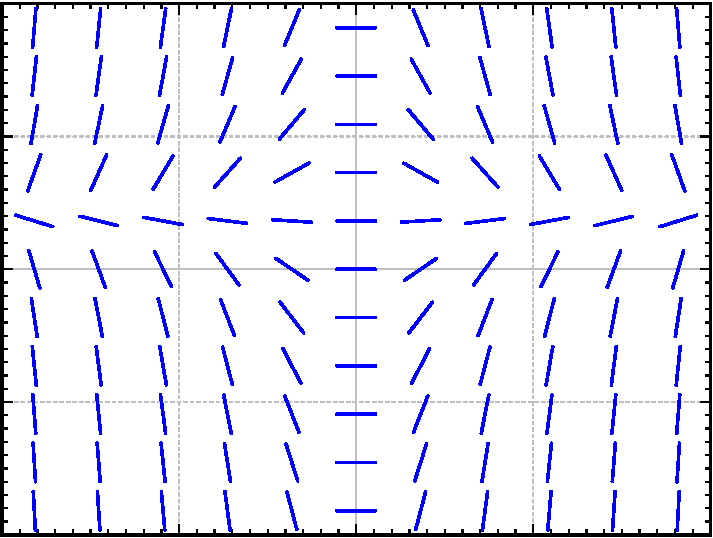
\includegraphics[width=1.75in]{figures/yprimex1minusyslope}}
\task
\parbox[c]{1.75in}{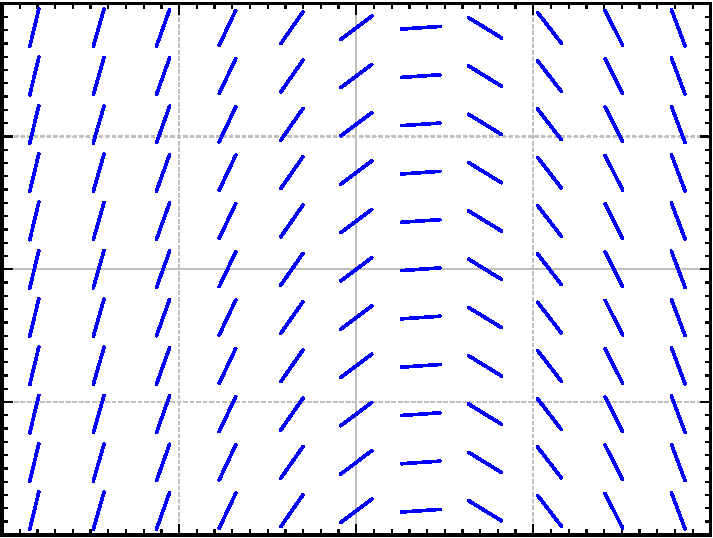
\includegraphics[width=1.75in]{figures/yprime1minusxslope}}
\task
\parbox[c]{1.75in}{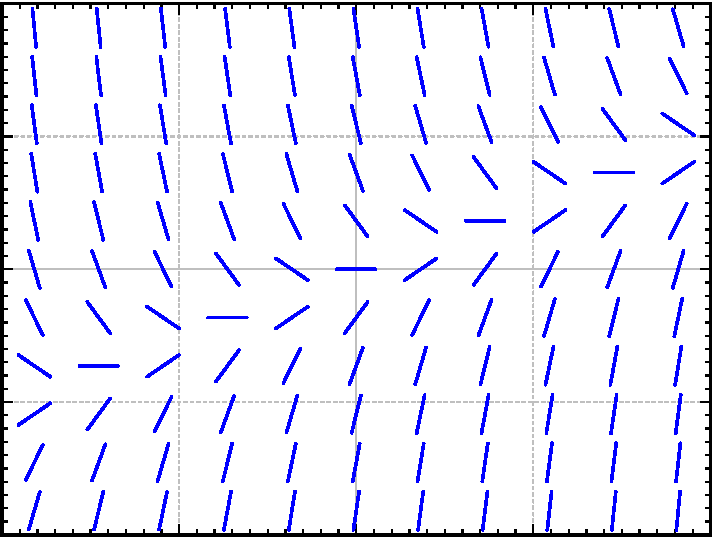
\includegraphics[width=1.75in]{figures/yprimexminus2yslope}}
\end{tasks}
\end{exercise}
\end{samepage}

\begin{exercise}[défi]
Soit $y' = f(x,y)$, $y(0) = 0$, tel que $f(x,y) > 1$
pour tous $x$ et $y$.   Si la solution existe  pour tout $x$,  que peut-on dire à propos de $y(x)$ lorsque $x$ tend vers l'infini?  Expliquez.
\end{exercise}

\begin{exercise}[défi]
Soit $(y-x)y' = 0$, $y(0) = 0$.
\begin{tasks}
\task Trouvez deux solutions distinctes.
\task Expliquez pourquoi ceci ne contredit pas le théorème de Picard.  
\end{tasks}
\end{exercise}

\begin{exercise}
Soit $y' = f(x,y)$.  Dites ce que vous savez à propos de son champ de directions, et dessinez un exemple, si vous avez l'information suivante à propos de  $f(x,y)$:
\begin{tasks}(2)
\task $f$ ne dépend pas de $y$.
\task $f$ ne dépend pas de $x$.
\task $f(t,t) = 0$ pour toute valeur $t$.
\task $f(x,0) = 0$ et $f(x,1) = 1$ pour tout $x$.
\end{tasks}
\end{exercise}

\begin{exercise}
Trouvez une solution à $y' = \lvert y \rvert$, $y(0) = 0$.  Peut-on appliquer le théorème de Picard?
\end{exercise}

\begin{exercise}
Soit $y' = (y-2x) g(x,y) + 2$, où $g(x,y)$ est une fonction quelconque.
Pouvez-vous résoudre l'équation avec condition initiale $y(0) = 0$,
et si oui, quelle est la solution?
\end{exercise}

\begin{exercise}[défi]
\pagebreak[2]
Soit $y' = f(x,y)$ tel que $f(x,1) = 0$ pour tout $x$,
$f$ est continue et $\frac{\partial f}{\partial y}$ existe et est continue pour tous $x$ et $y$.
\begin{tasks}
\task
Devinez une solution pour la condition initiale
$y(0) = 1$.
\task
Les graphes de deux solutions ayant des conditions initiales différentes peuvent-elles s'intersecter?
\task
En supposant que $y(0) = 0$, que peut-on dire à propos de la solution?  En particulier, peut-on avoir $y(x) > 1$ pour un certain $x$?  Peut-on avoir $y(x) = 1$ pour un certain  $x$?  Pourquoi ou pourquoi pas?
\end{tasks}
\end{exercise}

\setcounter{exercise}{100}

\begin{exercise}
Dessiner le champ de directions pour $y'=y^3$.  Pouvez-vous identifier visuellement une solution telle que $y(0)=0$?
\end{exercise}
\exsol{%
\\[6pt]
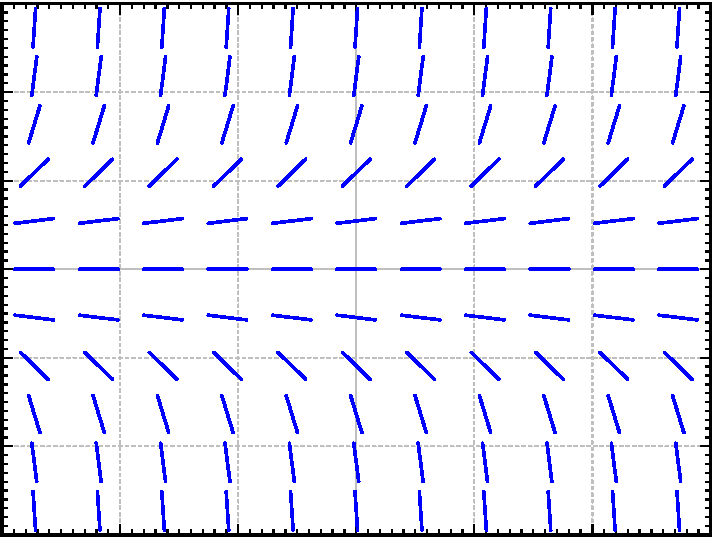
\includegraphics[width=2in]{figures/yprimey3slope}
\\
$y=0$ est une solution telle que $y(0)=0$.
}

\begin{exercise}
Est-il possible de résoudre $y' = xy$, $y(0) = 0$?  La solution est-elle unique?
\end{exercise}
\exsol{%
Oui une solution existe.  Car $y' = f(x,y)$ où $f(x,y) = xy$.  La fonction 
$f(x,y)$ est continue et 
$\frac{\partial f}{\partial y} = x$, qui est aussi continue près de $(0,0)$.
Par conséquent, la solution existe et est unique.  (En fait $y=0$ est une solution).
}

\begin{exercise}Peut-on résoudre $y' = \frac{x}{x^2-1}$, $y(1) = 0$?
\end{exercise}
\exsol{%
Non puisque la seule solution possible n'est pas définie au point $(x,y) = (1,0)$.
}

\begin{samepage}
\begin{exercise}
Associez les équations suivantes, $y'=\sin x$, $y'=\cos y$, $y' = y\cos(x)$ à leurs champs de directions respectifs.
Justifiez votre réponse.
\begin{tasks}(3)
\task
\parbox[c]{1.75in}{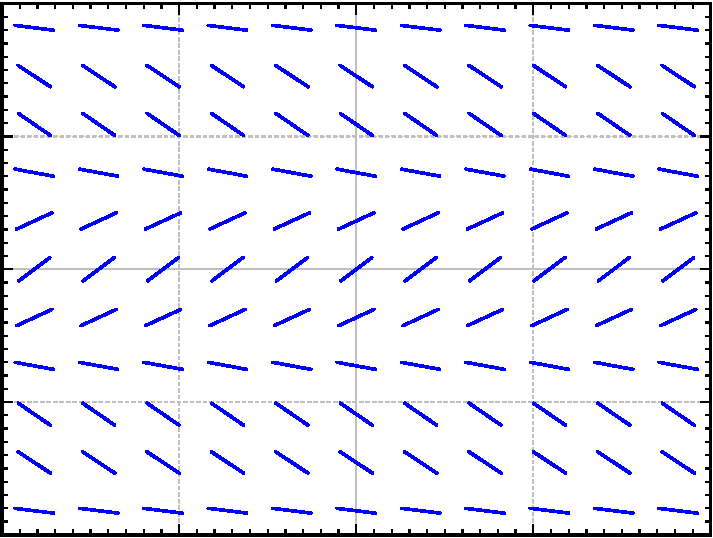
\includegraphics[width=1.75in]{figures/yprimecosyslope}}
\task
\parbox[c]{1.75in}{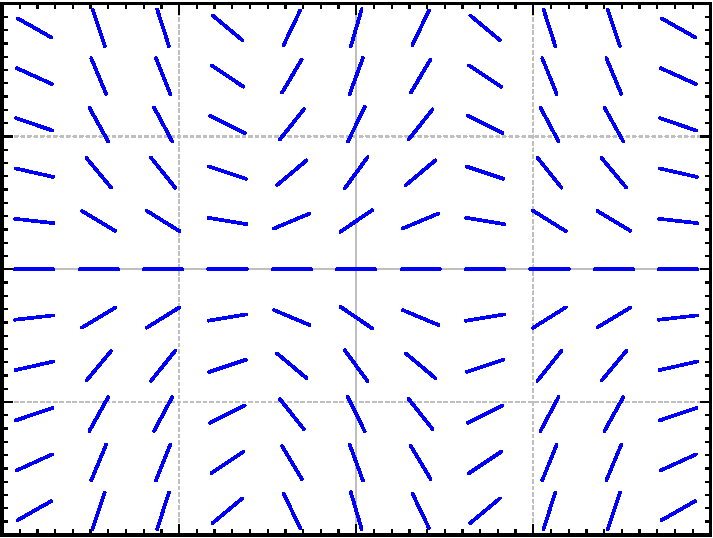
\includegraphics[width=1.75in]{figures/yprimecosxyslope}}
\task
\parbox[c]{1.75in}{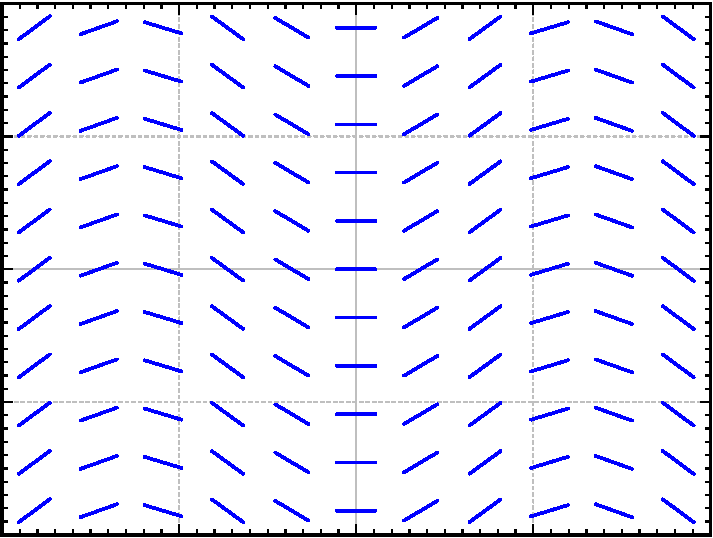
\includegraphics[width=1.75in]{figures/yprimesinxslope}}
\end{tasks}
\end{exercise}
\end{samepage}
\exsol{%
a) $y'=\cos y$, \quad
b) $y' = y\cos(x)$, \quad
c) $y'=\sin x$. \quad
%Justification left to reader.
}

\begin{exercise}[défi]
%[tricky]
Supposons que 
\begin{equation*}
f(y) =
\begin{cases}
0 & \text{ si $y > 0$}, \\
1 & \text{ si $y \leq 0$} .
\end{cases}
\end{equation*}
Est-ce que $y' = f(y)$, $y(0) = 0$ admet une solution dont la dérivée est continue?  Le théorème de Picard s'applique-t-il?  Pourquoi ou pourquoi pas?
\end{exercise}
\exsol{%
Picard ne s'applique pas puisque $f$ n'est pas continue en $y=0$.  
De plus, l'équation n'admet pas de solution dont la dérivée est continue.  Car si c'était vrai, alors il s'ensuivrait que
$y'(0) = 1$.  Par le test de la première dérivée, $y(x) > 0$ pour de petites valeurs positives de $x$.
Mais on a que $y'(x) = 0$ pour ces valeurs de $x$, et donc $y'$ n'est pas continue.
}
 
\begin{exercise}
Considérons une équation de la forme $y' = f(x)$, où $f$ est une fonction continue quelconque,vavec condition initiale $y(x_0) = y_0$.  Existe-t-il une solution pour tout $x$?  Pourquoi ou pourquoi pas?

\end{exercise}
\exsol{%
La solution est $y(x) = \int_{x_0}^x f(s) \,ds + y_0$, ce qui existe pour toute valeur de $x$.
}

%%%%%%%%%%%%%%%%%%%%%%%%%%%%%%%%%%%%%%%%%%%%%%%%%%%%%%%%%%%%%%%%%%%%%%%%%%%%%%

\sectionnewpage
\section{Les équations séparables}
\label{separable:section}

%\sectionnotes{1 lecture\EPref{, \S1.4 in \cite{EP}}\BDref{,
%\S2.2 in \cite{BD}}}

Lorsqu'une équation différentielle s'écrit sous la forme 
$y' = f(x)$,
il suffit d'intégrer pour en obtenir la solution\,:
$y = \int f(x) \,dx + C$. 
Malheureusement, cette technique ne fonctionne pas dans le cas général, c'est-à-dire 
$y' = f(x,y)$,
car si l'on intègre des deux côtés, on obtient\,: 
\begin{equation*}
y = \int f(x,y) \,dx + C .
\end{equation*}
Mais l'intégrale contient des termes en $y$, qu'on ne peut pas tout simplement \og{}traiter comme une constante\fg{}, puisque c'est une variable dépendante de $x$.

\subsection{Les équations séparables}

On dit qu'une équation différentielle est
\emph{\myindex{séparable}}
si elle peut être écrite sous la forme suivante\,: 
\begin{equation*}
	y' = f(x)g(y), 
\end{equation*}
où $f(x)$, $g(y)$ peuvent être des fonctions quelconques.
Écrivons cette équation à l'aide de la \myindex{notation de Leibniz}\,: 
\begin{equation*}
\frac{dy}{dx} = f(x)g(y) .
\end{equation*}
On peut alors réécrire l'équation comme suit\,: 
\begin{equation*}
\frac{dy}{g(y)} = f(x) \,dx .
\end{equation*}
Les deux côtés de l'équation sont des expressions qu'on peut intégrer\,: 
\begin{equation*}
\int \frac{dy}{g(y)} = \int f(x) \,dx + C .
\end{equation*}
Si l'on réussit à trouver des primitives de chaque côté, on pourra alors possiblement résoudre pour $y$.

\begin{example} \label{example:yprimeisxy}
Prenons l'équation  suivante\,: 
\begin{equation*}
y' = xy .
\end{equation*}
On observe que $y=0$ est une solution.  Nous gardons cette solution en mémoire et supposons maintenant que 
$y \not =0$, ce qui nous permettra de diviser par $y$.
Écrivons l'équation comme suit\,: $\frac{dy}{dx} = xy$.  On intègre de chaque côté\,: 
\begin{equation*}
\int \frac{dy}{y} = \int x\,dx + C .
\end{equation*}
On calcule les primitives de chaque côté et l'on obtient\,:
\begin{equation*}
\ln \, \lvert y\rvert = \frac{x^2}{2} + C 
\end{equation*}
ou
\begin{equation*}
\lvert y \rvert = e^{\frac{x^2}{2} + C} = e^{\frac{x^2}{2}} e^C = D e^{\frac{x^2}{2}} ,
\end{equation*}
où $D > 0$ est une constante.  Puisque $y=0$ est aussi une solution et que, de plus, on a la valeur absolue de $y$, dans l'expression, on peut écrire\,: 
%
\begin{equation*}
y = D e^{\frac{x^2}{2}} ,
\end{equation*}
où $D$ est une constante quelconque, pouvant être 0 ou négative.  Vérifions que c'est une solution\,: 
\begin{equation*}
y' = D x e^{\frac{x^2}{2}} = x \left( D e^{\frac{x^2}{2}} \right) = xy .
\end{equation*}
\end{example}

Regardons de plus près cette méthode.  On pourrait s'inquiéter du fait que les deux intégrales apparaissant dans l'expression soient en termes de variables différentes.  Ça peut sembler erroné... Alors, nous allons revoir la méthode de séparation des variables de manière plus rigoureuse.

Supposons donc qu'on a: 
\begin{equation*}
\frac{dy}{dx} = f(x)g(y) .
\end{equation*}
Observons que $y = y(x)$ est une fonction de $x$ et que
$\frac{dy}{dx}$ l'est également.  On peut donc réécrire l'équation comme suit\,: 
\begin{equation*}
\frac{1}{g(y)}\,\frac{dy}{dx} = f(x) .
\end{equation*}
Maintenant, intégrons les deux côtés par rapport à $x$\,: 
\begin{equation*}
\int \frac{1}{g(y)}\,\frac{dy}{dx} \,dx = \int f(x) \,dx + C .
\end{equation*}
On fait un changement de variables dans l'intégrale de gauche\,: 
\begin{equation*}
\int \frac{1}{g(y)}\,dy = \int f(x) \,dx + C .
\end{equation*}
Comme on peut voir, on obtient la même formule que plus haut, qui est donc correcte.

\subsection{Les solutions implicites}

Parfois, on peut avoir de la difficulté avec la méthode des équations séparables, même si les deux intégrales sont résolubles.  Considérons, par exemple, l'équation séparable suivante: 
\begin{equation*}
y' = \frac{xy}{y^2+1} .
\end{equation*}
On sépare les variables\,: 
\begin{equation*}
\frac{y^2+1}{y}\,dy = \left(y+\frac{1}{y}\right)\,dy = x\,dx .
\end{equation*}
On intègre\,: 
\begin{equation*}
\frac{y^2}{2} + \ln \, \lvert y \rvert = \frac{x^2}{2} + C. 
\end{equation*}
Puis on réécrit pour rendre la solution plus jolie (ici, $D = 2C$): 
\begin{equation*}
y^2 + 2 \ln \, \lvert y\rvert = x^2 + D .
\end{equation*}
Il est difficile de trouver une expression explicite pour $y$, puisqu'on ne peut pas l'isoler dans l'expression.  Dans un tel cas, on obtient ce qu'on appelle une 
\emph{\myindex{solution implicite}}.
On peut tout de même vérifier qu'on a bien trouvé une solution à l'équation différentielle.  Il suffit de dériver chaque côté par rapport à $x$, en se souvenant que $y$ est une fonction de $x$, et l'on obtient: 
\begin{equation*}
	y'\left(2y + \frac{2}{y}\right) = 2x .
\end{equation*}
En multipliant les deux côtés par $y$ et en divisant par $2(y^2+1)$, on retrouve l'équation différentielle de départ (vérifiez-le).

Étant donné une solution implicite, trouver des valeurs de $y$ explicitement peut être difficile.  Il est possible qu'une valeur de $x$ donne plusieurs valeurs possibles de $y$, et qu'il faille alors choisir.  Parfois, il est plus simple de penser à $x$ comme une fonction de $y$.  Parfois, même ceci est difficile.

Dans ce cas, un ordinateur peut être votre ami.  La plupart des logiciels mathématiques proposent une fonction pour tracer la courbe-solution d'une équation implicite.  Par exemple, pour $C=0$, l'ensemble des points $(x,y)$ satisfaisant à $y^2+2\ln|y|=x^2$ 
est une union de deux courbes, illustrées à la \figureref{implicitsols:fig}.  Ce n'est pas le graphe d'une fonction, puisque chaque $x$ admet deux valeurs possibles de $y$.  Mais si l'on choisit une des deux courbes, on a alors le graphe d'une fonction.  Si, de plus, on a une condition initiale, on choisit la courbe qui passe par ce point.  Ainsi, chaque valeur de $C$ donne deux solutions.  Comme on peut le voir, les solutions implicites ne sont pas simples, mais parfois on ne peut pas obtenir mieux.

\begin{myfig}
\capstart
\diffyincludegraphics{width=3in}{width=4.5in}{implicitsols}
\caption{Solution implicite $y^2+2\ln|y|=x^2$ à l'équation $y'=\frac{xy}{y^2+1}$.\label{implicitsols:fig}}
\end{myfig}

Cet exemple admet aussi la solution $y=0$.
Ainsi, la solution générale est 
\begin{equation*}
	y^2 + 2 \ln \, \lvert y \rvert = x^2 + C \qquad \text{ou} \qquad y=0.
\end{equation*}
Des solutions comme $y=0$
sont parfois appelées des \emph{solutions singulières\index{solutions singulières}}.

\subsection{Exemples d'équations séparables}

\begin{example}
Résolvons $x^2y' = 1 - x^2+y^2 - x^2y^2$, $y(1) = 0$.

On factorise le côté droit: 
\begin{equation*}
x^2y' = (1 - x^2)(1+y^2).
\end{equation*}
On sépare les variables, on intègre et l'on résout pour $y$\,: 
\begin{align*}
\frac{y'}{1+y^2} & = \frac{1 - x^2}{x^2} , \\
\frac{y'}{1+y^2} & = \frac{1}{x^2} - 1 , \\
\operatorname{arctan} (y) & = \frac{-1}{x} - x + C , \\
y & = \tan \left(\frac{-1}{x} - x + C\right) .
\end{align*}
Il reste à résoudre pour la condition initiale,
 $0 = \tan(-2+C)$, et l'on obtient $C=2$ (ou $C = 2 +
\pi$, ou $C = 2 + 2\pi$, etc.).  La solution particulière recherchée est donc
\begin{equation*}
y = \tan \left(\frac{-1}{x} - x + 2 \right) .
\end{equation*}
\end{example}

\begin{example} \label{sep:coffeeexample}
Alex se prépare une tasse de café, qui doit se rendre à 60 degrés (Celsius) parce qu'Alex n'aime pas se brûler.  Initialement, à $t=0$ minute,
le café était à 89 degrés.  Une minute plus tard, Alex mesure la température de nouveau, et c'est 85 degrés.  La température ambiante est 22 degrés.  Quand est-ce qu'Alex pourra enfin déguster son café?

Posons $T$, la température du café en degrés Celsius, et $A$, la température ambiante, toujours en degrés Celsius. La 
\myindex{loi de refroidissement de Newton} affirme que le taux de changement de la température du café est proportionnel à la différence entre la température du café et la température ambiante.  Autrement dit\,: 
%
\begin{equation*}
\frac{dT}{dt} = k(A-T), 
\end{equation*}
où $k$ est une constante.
Dans notre exemple\,: $A=22$, $T(0) = 89$, $T(1) = 85$.
On sépare les variables et l'on intègre (ici, $C$ et $D$ sont des constantes arbitraires):
\begin{align*}
\frac{1}{T-A} \, \frac{dT}{dt} & = -k , \\
\ln (T-A) &= -kt + C , \qquad \text{(notons que } T-A > 0 \text{)} \\
T-A &= D\, e^{-kt} ,  \\
T &= A + D\, e^{-kt} .
\end{align*}
En substituant la valeur de $A$, on a 
$T = 22 + D\, e^{-kt}$.  On substitue la condition initiale\,: $89 = T(0) = 22 +
D$,
et donc $D = 67$.  Ainsi, 
$T = 22 + 67\, e^{-kt}$.  La deuxième condition donne que $85 = T(1) = 
22 + 67\, e^{-k}$.  En résolvant pour $k$, on obtient 
$k = - \ln \frac{85-22}{67} \approx 0,0616$.  Maintenant, trouvons la valeur de $t$ donnant une température de 60 degrés.  On résout l'équation suivante, 
\begin{equation*}
	60 = 22 + 67 e^{-0,0616t}
\end{equation*}
pour obtenir 
$t = - \frac{\ln \frac{60-22}{67}}{0,0616} \approx 9,21$ minutes.  Donc, Alex peut commencer à boire son café environ 9 minutes après l'avoir préparé (correspondant à peu près au temps requis pour faire ce calcul).  Voir la \figureref{sintro:coffeefig}.




	%%%%%JP rendu ici 2023-02-24






\begin{myfig}
\capstart
%original files coffeefig-1 coffeefig-2
\diffyincludegraphics{width=6.24in}{width=9in}{coffeefig-1-2}
\caption{Graphes de la fonction de température du café $T(t)$.
À gauche, des droites horizontales sont tracées aux températures 60, 85, et 89.  Des droites verticales sont tracées à $t=1$ et $t=9.21$.  Observez que la température atteint la valeur 85 à $t=1$, et 60 à 
$t \approx 9.21$.  À droite, le graphe montre la température pour une plus longue durée, avec une droite horizontale à la valeur de la température ambiante, soit 22.\label{sintro:coffeefig}}
\end{myfig}
\end{example}

\begin{example}
Trouvons la solution générale de $y' = \frac{-xy^2}{3}$ (incluant les solutions singulières).

Notons d'abord que $y=0$ est une solution (singulière).
Supposons donc pour la suite que $y \not= 0$.  On sépare les variables et on intègre\,: 
\begin{align*}
\frac{-3}{y^2} y' & = x  \displaybreak[0]\\
\frac{3}{y} & = \frac{x^2}{2} + C  \displaybreak[0]\\
y & = \frac{3}{\nicefrac{x^2}{2} + C}
= \frac{6}{x^2 + 2C}.
\end{align*}
La solution générale est donc 
\begin{align*}
y = \frac{6}{x^2 + 2C} \qquad \text{ou} \qquad y=0 .
\end{align*}
\end{example}

\subsection{Exercices}

\begin{exercise}
Résolvez $y' = \nicefrac{x}{y}$.
\end{exercise}

\begin{exercise}
Résolvez$y' = x^2y$.
\end{exercise}

\begin{exercise}
Résolvez $\dfrac{dx}{dt} = (x^2-1)\,t$, $x(0) = 0$.
\end{exercise}

\begin{exercise}
Résolvez $\dfrac{dx}{dt} = x\,\sin(t)$, for $x(0) = 1$.
\end{exercise}

\begin{exercise}
Résolvez $\dfrac{dy}{dx} = xy+x+y+1$.  Indice\,: factorisez le côté droit.
\end{exercise}

\begin{exercise}
Résolvez $xy' = y + 2x^2 y$, $y(1) = 1$.
\end{exercise}

\begin{exercise}
Résolvez$\dfrac{dy}{dx} = \dfrac{y^2+1}{x^2+1}$, $y(0) = 1$.
\end{exercise}

\begin{exercise}
Trouvez une solution implicite pour
$\dfrac{dy}{dx} = \dfrac{x^2+1}{y^2+1}$, $y(0) = 1$.
\end{exercise}

\begin{exercise}
Trouvez une solution explicite pour $y' = xe^{-y}$, $y(0)=1$.
\end{exercise}

\begin{exercise}
Trouvez une solution explicite pour $xy' = e^{-y}$, $y(1)=1$.
\end{exercise}

\begin{exercise}
Trouvez une solution explicite pour $y' = ye^{-x^2}$, $y(0)=1$.  Au besoin, votre réponse peut inclure une intégrale.
\end{exercise}

\begin{exercise}
Supposons qu'une tasse de café est à 100 degrés Celsius au temps $t=0$,
et 70 degrés à $t=10$ minutes, et 50 degrés à $t=20$
minutes.  Calculez la température ambiante.
\end{exercise}

\setcounter{exercise}{100}

\begin{exercise}
Résolvez $y'=2xy$.
\end{exercise}
\exsol{%
$y = Ce^{x^2}$
}

\begin{exercise}
Résolvez $x'=3xt^2-3t^2$, $x(0)=2$.
\end{exercise}
\exsol{%
$x = e^{t^3}+1$
}

\begin{exercise}
Trouvez une solution implicite pour 
$x'=\frac{1}{3x^2+1}$, $x(0)=1$.
\end{exercise}
\exsol{%
$x^3+x=t+2$
}

\begin{exercise}
Trouvez une solution explicite pour $x y' = y^2$, $y(1) = 1$.
\end{exercise}
\exsol{%
$y = \frac{1}{1-\ln x}$
}

\begin{exercise}
Trouvez une solution implicite pour $y' = \frac{\sin(x)}{\cos(y)}$.
\end{exercise}
\exsol{%
$\sin(y) = -\cos(x) + C$
}

\begin{exercise}
Reprenez l'\exampleref{sep:coffeeexample} avec les mêmes valeurs\,: 89 degrés à 
$t=0$, 85 degrés à $t=1$, et une température ambiante de 22 degrés. 
Supposons que ces températures ont été mesurées avec une précision de 
$\pm 0.5$ degrés.  À cause de cette imprécision, on ne connaît qu'un intervalle de temps pour que la température du 
café atteigne exactement 60 degrés.  Trouvez cet intervalle de temps.  Indice\,: quel type d'erreur rend le temps de refroidissement plus long? Plus court? 
\end{exercise}
\exsol{%
L'intervalle de temps est d'environ 7.45 à 12.15 minutes.
}

\begin{exercise}
Une population de lapins $x$ sur une île est modelisée par l'équation suivante\,: 
$x' = x- \bigl(\nicefrac{1}{1000} \bigr) x^2$, où la variable indépendante $t$ est le temps, mesuré en mois.  À  $t=0$, l'île contient 40 lapins.
\begin{tasks}
\task Résolvez l'équation différentielle avec condition initiale.
\task 
Combien de lapins habitent l'île après 1 mois, 5 mois, 10 mois, 15 mois?  Arrondissez à l'entier le plus proche.
\end{tasks}
\end{exercise}
\exsol{%
a) $x = \frac{1000e^t}{e^t+24}$. \quad b) 102 lapins après un mois,
861 après 5 mois, 999 après 10 mois, 1000 après 15 mois.
}

%%%%%%%%%%%%%%%%%%%%%%%%%%%%%%%%%%%%%%%%%%%%%%%%%%%%%%%%%%%%%%%%%%%%%%%%%%%%%%

\sectionnewpage
\section{Les équations linéaires et le facteur intégrant}
\label{intfactor:section}

%\sectionnotes{1 lecture\EPref{, \S1.5 in \cite{EP}}\BDref{,
%\S2.1 in \cite{BD}}}

Les \emph{équations linéaires\index{équation linéaire}} sont parmi les équations différentielles les plus importantes à comprendre.  Une bonne partie des équations que nous voyons dans ce manuel sont en fait linéaires.  Cette section est dédiée aux \emph{\myindex{équations linéaires du premier ordre}}.
Une équation du premier ordre est dite linéaire si elle peut s'écrire sous la forme suivante :
\begin{equation} \label{lineq:eq1}
y' + p(x) y = f(x) .
\end{equation}
Être "linéaire" veut dire que l'expression est linéaire en $y$ et $y'$; l'équation ne contient pas de puissances plus élevées ni d'autres fonctions de $y$ ou $y'$.
Cependant, la dépendance sur la variable $x$ peut être plus compliquée.

La raison qu'on aime les équations linéaires c'est qu'elles ont de belles propriétés.  Par exemple, la solution existe pour tout $x$ où $p(x)$ and $f(x)$ sont définies (voir de plus la remarque~\ref{rem:regular}).  Ce qui nous intéressera surtout, à ce stade-ci, c'est qu'il y a une méthode générale pour résoudre les équations linéaires du premier ordre.

L'idée\,: ré-écrire le côté gauche de  \eqref{lineq:eq1} comme une dérivée du produit de $y$ avec une fonction à déterminer.  Ainsi nous cherchons une fonction $r(x)$ telle que \,:
\begin{equation*}
r(x) y' + r(x) p(x) y = \frac{d}{dx}\Bigl[ r(x) y \Bigr] .
\end{equation*}
Ceci est le côté gauche de 
\eqref{lineq:eq1} multiplié par $r(x)$.  Donc si on multiplie \eqref{lineq:eq1} par
$r(x)$, on obtient\,:
\begin{equation*}
\frac{d}{dx}\Bigl[ r(x) y \Bigr] = r(x)f(x) .
\end{equation*}
Maintenant, on intègre les deux côtés. 
C'est possible puisque le côté droit ne dépend pas de $y$ et le côté gauche est la dérivée d'une fonction.  Ensuite, on résoud pour  $y$.
La fonction $r(x)$ s'appelle le \emph{\myindex{facteur intégrant}} et la méthode s'appelle la 
\emph{\myindex{méthode du facteur intégrant}}.

Comment trouver $r(x)$?  On cherche une fonction qui, lorsqu'on la dérive, on obtient de nouveau la fonction, multipliée par $p(x)$.  Les fonctions exponentielles ont précisément cette propriété.  On pose donc\,: 
%
\begin{equation*}
r(x) = e^{\int p(x) \,dx} .
\end{equation*}
On substitue cette valeur dans l'équation différentielle pour obtenir ce qui suit\,: 
\begin{align*}
y' + p(x) y &= f(x) , \\
e^{\int p(x) \,dx} y' + e^{\int p(x) \,dx} p(x) y & = e^{\int p(x) \,dx} f(x) , \\
\frac{d}{dx}\left[ e^{\int p(x) \,dx} y \right] & = e^{\int p(x) \,dx} f(x) , \\
e^{\int p(x) \,dx} y & = \int e^{\int p(x) \,dx} f(x) \,dx + C , \\
y & = e^{-\int p(x) \,dx} \left( \int e^{\int p(x) \,dx} f(x) \,dx + C \right) .
\end{align*}

On pourra obtenir une formule analytique pour $y$, à condition de pouvoir trouver les primitives de chacune des intégrales apparaissant dans l'expression.

\begin{example}
Résolvons 
\begin{equation*}
y' + 2xy = e^{x-x^2}, \qquad y(0) = -1 .
\end{equation*}

Notons d'abord que $p(x) = 2x$ et $f(x) = e^{x-x^2}$.
Le facteur intégrant est $r(x) = e^{\int p(x)\, dx} = e^{x^2}$.
On multiplie chaque côté de l'équation par $r(x)$ pour obtenir\,:
\begin{align*}
e^{x^2} y' + 2xe^{x^2}y & = e^{x-x^2} e^{x^2} , \\
\frac{d}{dx} \left[ e^{x^2} y \right] &= e^x .
\end{align*}
On intègre\,: 
\begin{align*}
e^{x^2} y &= e^x +C , \\
y &= e^{x-x^2} + C e^{-x^2} .
\end{align*}
Ensuite, on résoud pour la condition initiale $-1 = y(0) = 1 + C$, ce qui donne $C=-2$.
La solution est donc\,:
\begin{equation*}
y = e^{x-x^2} - 2 e^{-x^2} .
\end{equation*}
\end{example}
Notons qu'on peut prendre la primitive de notre choix pour 
$e^{\int p(x) dx}$.  On peut rajouter une constante d'intégration, mais ça ne changera pas la réponse à la fin.

\begin{exercise}
Essayez-le\,: ajoutez une constante d'intégration au facteur intégrant dans l'exemple et vérifiez que vous obtenez la même solution qu'ici.
\end{exercise}

Conseil\,: Plutôt que d'apprendre par coeur la formule, retenez plutôt la méthode pour l'obtenir.  C'est plus simple et il suffit alors de répéter la méthode pour résoudre le problème. 

Puisqu'on ne peut pas toujours trouver une solution analytique, il peut être utile de savoir comment écrire la solution sous forme d'intégrale définie.  Car une intégrale définie peut être traitée par un logiciel de calcul.  Soit l'équation suivante\,:
\begin{equation*}
y' + p(x) y = f(x) , \qquad y(x_0) = y_0 .
\end{equation*}
Écrivons la solution sous forme d'intégrale définie 
\begin{equation} \label{lei:defsol}
\mybxbg{
~~
y(x) = e^{-\int_{x_0}^x p(s)\, ds} \left( \int_{x_0}^x e^{\int_{x_0}^t p(s)\, ds}
f(t) \,dt + y_0 \right).
~~
}
\end{equation}
Cette formule peut maintenant être lue par une application de calcul numérique, en la codant convenablement.

\begin{exercise}
Vérifiez que $y(x_0) = y_0$ dans \eqref{lei:defsol}.
\end{exercise}

\begin{exercise}
Écrivez la solution du problème suivant sous forme d'intégrale définie.  Vous ne pourrez pas trouver une solution analytique à cette équation.
%
\begin{equation*}
y' + y = e^{x^2-x}, \qquad y(0) = 10 .
\end{equation*}
\end{exercise}

\begin{remark}\label{rem:regular}
Avant de continuer, notons quelques propriétés intéressantes des équations linéaires.  D'abord, il existe toujours une formule explicite \eqref{lei:defsol} pour la 
solution de l'équation à condition initiale 
$y' + p(x) y = f(x)$, $y(x_0) = y_0$.  Deuxièmement, la formule 
\eqref{lei:defsol} implique que si $p(x)$
et $f(x)$ sont continues sur un intervalle $(a,b)$, alors la solution 
$y(x)$ existe et est différentiable sur $(a,b)$.  Comparez à l'exemple non-linéaire vu précédemment, $y'=y^2$,
ainsi qu'au \thmref{slope:picardthm}.
\end{remark}


\begin{example}
Voyons maintenant une application des équations linéaires qui est couramment rencontrée\,: la concentration de produits chimiques dans un plan d'eau.

\begin{mywrapfigsimp}{1.60in}{1.65in}
\noindent
\inputpdft{lin-tank}
\end{mywrapfigsimp}
Un réservoir d'une capacité de 100 litres contient 10 kilogrammes de sel dissout dans 60 litres d'eau.  Une solution d'eau saline avec une concentration de 0.1 kilogrammes par litre entre dans le réservoir à un taux de 5 litres par minute. La solution dans le réservoir est bien brassée (c'est-à-dire, on peut supposer que la concentration est la même partout) et sort à un taux de 3 litres par minute.  Combien de sel est contenu dans le réservoir lorsqu'il est plein?

Commençons par établir l'équation différentielle modélisant ce problème.  Dénotons par $x$ la quantité de sel dans le réservoir, en kilogrammes,  et par $t$ le temps en minutes.  Si on considère une petite variation $\Delta t$ dans le temps, la variation en $x$ (dénotée $\Delta x$) est approximativement \,: 
\begin{equation*}
\Delta x \approx
(\text{taux entrée} \times \text{concentration entrée}) \Delta t - 
(\text{taux sortie} \times \text{concentration sortie}) \Delta t .
\end{equation*}
On divise partout par $\Delta t$ et on prend la limite $\Delta t \to 0$ pour obtenir\,: 
\begin{equation*}
\frac{dx}{dt} =
(\text{taux entrée} \times \text{concentration entrée})  - 
(\text{taux sortie} \times \text{concentration sortie}) .
\end{equation*}
Dans notre exemple\,:
\begin{align*}
\text{taux entrée} &= 5 , \\
\text{concentration entrée} &= 0.1 , \\
\text{taux sortie} &= 3 , \\
\text{concentration sortie} &= \frac{x}{\text{volume}} = \frac{x}{60+(5-3)t} .
\end{align*}
L'équation modélisant le problème est donc\,: 
\begin{equation*}
\frac{dx}{dt} =
(5 \times 0.1)  - 
\left(3 \frac{x}{60+2t}\right) .
\end{equation*}
On ré-écrit ceci sous la forme \eqref{lineq:eq1}\,:
\begin{equation*}
\frac{dx}{dt} +
\frac{3}{60+2t} x
=
0.5 .
\end{equation*}

Maintenant on peut résoudre l'équation.  Le facteur intégrant est\,:  
\begin{equation*}
r(t) = \exp \left( \int \frac{3}{60+2t} dt  \right)
=
\exp \left( \frac{3}{2} \ln (60+2t) \right)
=
{(60+2t)}^{3/2} .
\end{equation*}

On multiplie les deux côtés de l'équation par le facteur intégrant, et on obtient\,: 
\begin{align*}
{(60+2t)}^{3/2} \frac{dx}{dt} +
{(60+2t)}^{3/2} \frac{3}{60+2t} x
& =
0.5{(60+2t)}^{3/2} \\
\frac{d}{dt}\left[
{(60+2t)}^{3/2} x \right]
& =
0.5{(60+2t)}^{3/2} \\
{(60+2t)}^{3/2} x
& =
\int 
0.5{(60+2t)}^{3/2}
dt
+C \\
 x
& =
{(60+2t)}^{-3/2} \int 
\frac{
{(60+2t)}^{3/2}
}{2}
dt
+C{(60+2t)}^{-3/2} \\
 x
& =
{(60+2t)}^{-3/2}
\frac{1}{10}{(60+2t)}^{5/2}
+C{(60+2t)}^{-3/2} \\
 x
& =
\frac{60+2t}{10}
+C{(60+2t)}^{-3/2} .
\end{align*}

%mbxSTARTIGNORE
\begin{mywrapfig}{3.25in}
\capstart
\diffyincludegraphics{width=3in}{width=4.5in}{linear-salt-graph}
\caption{Graphe de la solution $x$ kilogrammes de sel dans le réservoir au temps 
$t$.\label{linear-salt-graph:fig}}
\end{mywrapfig}
%mbxENDIGNORE
%
% Make sure to keep the above and the mbx figure below in sync!
%
On doit trouver la valeur de $C$.  On sait qu'à $t=0$, $x=10$.  Donc\,: 
\begin{equation*}
10 = x(0)
=
\frac{60}{10}
+C{(60)}^{-3/2}
=
6
+C{(60)}^{-3/2} ,
\end{equation*}
ou
\begin{equation*}
C=4 ({60}^{3/2}) \approx 1859.03 .
\end{equation*}

On cherche à savoir la valeur de $x$ lorsque le réservoir est plein.  Ceci arrive lorsque $60+2t = 100$, c'est-à-dire à  $t=20$.  Donc
\begin{equation*}
\begin{split}
x(20) & = 
\frac{60+40}{10}
+C{(60+40)}^{-3/2}
\\
& \approx
10
+1859.03 {(100)}^{-3/2}
\approx
11.86 .
\end{split}
\end{equation*}
Voir la \figureref{linear-salt-graph:fig} pour le graphe de $x$ en fonction de $t$.

La concentration dans le réservoir plein est approximativement 
\unitfrac[0.1186]{kg}{litre}, alors que la concentration initiale est 
$\nicefrac{1}{6}$ ou \unitfrac[0.167]{kg}{litre}.
%mbxlatex \begin{myfig}
%mbxlatex \capstart
%mbxlatex \diffyincludegraphics{width=3in}{width=4.5in}{linear-salt-graph}
%mbxlatex \caption{Graph of the solution $x$ kilograms of salt in the tank at time
%mbxlatex $t$.\label{linear-salt-graph:fig}}
%mbxlatex \end{myfig}
\end{example}

\subsection{Exercices}

Dans les exercices suivants, n'hésitez pas à laisser la réponse sous forme d'intégrale définie si une solution analytique n'est pas possible.  Mais si la solution analytique existe, c'est celle-là que vous devriez donner.

\begin{exercise}
Résolvez $y' + xy = x$.
\end{exercise}

\begin{exercise}
Résolvez $y' + 6y = e^x$.
\end{exercise}

\begin{exercise}
Résolvez $y' + 3x^2y = \sin(x) \, e^{-x^3}$, $y(0) = 1$.
\end{exercise}

\begin{exercise}
Résolvez $y' + \cos (x) y = \cos(x)$.
\end{exercise}

\begin{exercise}
Résolvez $\frac{1}{x^2+1} \, y' + x y = 3$, $y(0) = 0$.
\end{exercise}

\begin{exercise}
Supposons que deux lacs se trouvent sur le plan d'un ruisseau. De l'eau propre s'écoule dans le premier lac, ensuite l'eau s'écoule du premier lac au deuxième lac, et enfin l'eau se déverse en aval du ruisseau à partir du deuxième lac. Le débit à l'entrée et à la sortie de chaque lac est 500 litres par heure.  Le premier lac contient 100 000 litres d'eau et le deuxième lac en contient 200 000.  Un camion déverse \unit[500]{kg} d'une matière dangereuse.  On suppose que l'eau est bien brassée par le ruisseau.
\begin{tasks}
\task Trouvez la concentration de la matière dangereuse dans chacun des lacs, en fonction du temps.
\task À quel moment est-ce que la 
concentration dans le premier lac tombe en-dessous de  \unit[0.001]{kg} par litre?
\task À quel moment est-ce que la concentration dans le deuxième sera maximale?
\end{tasks}
\end{exercise}

\begin{exercise}
La \myindex{loi de refroidissement de Newton} affirme que $\frac{dx}{dt} = -k(x-A)$, où 
$x$ est la température, $t$ est le temps, $A$ est la température ambiante,
et $k > 0$ est une constante.
Supposons que $A = A_0 \cos (\omega t)$, où $A_0$ et $\omega$ sont des constantes.  Autrement dit, la température ambiante oscille en fonction du temps (par exemple, varie entre le jour et la nuit).
\begin{tasks}
\task Trouvez la solution générale.
\task Est-ce que les conditions initiales ont un impact sur le comportement à long terme de la solution?  Pourquoi ou pourquoi pas?
\end{tasks}
\end{exercise}

\begin{exercise}
Un réservoir contient 5 grammes de sel dissous dans 20 litres d'eau.  Une solution saline, dont la concentration est de 2 grammes par litre, s'y déverse à un taux de 3 litres par minute.  Le contenu du réservoir est bien brassé et en ressort à un taux de 3 litres par minute. Quelle doit être la durée du procédé pour obtenir 20 grammes de sel dans le réservoir?
\end{exercise}

\begin{exercise}
Un réservoir contient 10 litres d'eau propre.  Une solution saline, de concentration inconnue mais constante, se déverse dans le réservoir à un taux de 1 litre par minute.  Le contenu du réservoir est bien brassé et en ressort à un taux de 1 litre par minute.  Au bout de 20 minutes, le réservoir contient 15 grammes de sel.  Quelle est la concentration de la solution saline entrante?
\end{exercise}

\setcounter{exercise}{100}

\begin{exercise}
Résolvez $y'+3 x^2 y = x^2$.
\end{exercise}
\exsol{%
$y = C e^{-x^3} + \nicefrac{1}{3}$
}

\begin{exercise}
Résolvez $y'+ 2\sin(2x) y = 2\sin(2x)$, $y(\nicefrac{\pi}{2}) = 3$.
\end{exercise}
\exsol{%
$y = 2 e^{\cos(2x)+1} + 1$
}

\begin{exercise}
Un réservoir d'eau est vidé à un taux de \unitfrac[3]{L}{min}.  Au départ, le réservoir contient \unit[10]{L} d'eau propre.  De l'eau contenant une matière dangereuse se déverse dans le réservoir à un taux de \unitfrac[2]{L}{min},
ave une concentration de \unitfrac[$20t$]{g}{L} au temps $t$.
Au moment où le réservoir est à moitié vide, combien de grammes de matière dangereuse sont contenus dans le réservoir?  (On suppose que c'est bien brassé.)
\end{exercise}
\exsol{%
$250$ grammes
}

\begin{exercise}
Supposons qu'on ait une population de bactéries à laquelle on ajoute graduellement une substance toxique, de telle sorte que le taux de croissance diminue.  Plus précisément, $\frac{dP}{dt} = (2-0.1\,t)P$.  Si $P(0) = 1000$, trouvez la population pour $t=5$.
\end{exercise}
\exsol{%
$P(5) = 1000 e^{2 \times 5 - 0.05 \times {5}^2} = 1000 e^{8.75} \approx
6.31 \times {10}^6$
}

\begin{exercise}
De l'eau se déverse dans un réservoir cylindrique à un débit de $d$ mètres cube par seconde.  Soit $A$ l'aire d'une section transversale du réservoir, en mètres.  Supposons que l'eau sort du réservoir à un débit qui est proportionnel à la hauteur du niveau d'eau.  Trouvez l'équation différentielle décrivant $h$, la hauteur du niveau d'eau, en introduisant les constantes dont vous avez besoin.  Donnez aussi les unités pour vos constantes.
\end{exercise}
\exsol{%
$Ah' = d - kh$, où $k$ est une constante mesurée en $\unit{m^2}{s}$.
}


%%%%%%%%%%%%%%%%%%%%%%%%%%%%%%%%%%%%%%%%%%%%%%%%%%%%%%%%%%%%%%%%%%%%%%%%%%%%%%

\sectionnewpage
\section{Les équations autonomes}
\label{auteq:section}

%\sectionnotes{1 lecture\EPref{, \S2.2 in \cite{EP}}\BDref{,
%\S2.5 in \cite{BD}}}

Considérons une équation différentielle comme suit\,:  
\begin{equation*}
\frac{dx}{dt} = f(x) 
\end{equation*}
où la dérivée dépend uniquement de $x$, la variable dépendante, et non de $t$, la variable indépendante.  De telles équations sont dites \emph{autonomes\index{équation autonome}}.  On dit "autonome" parce que, si on pense à la variable indépendante comme étant le temps, la valeur de la dérivée à un point est la même à tout moment.

Reprenons par exemple le problème du café qui tiédit 
(\exampleref{sep:coffeeexample}).
\myindex{La loi de refroidissement de Newton}
est une équation autonome\,: 
\begin{equation*}
\frac{dx}{dt} = k (A-x) 
\end{equation*}
où $x$ est la température, $t$ le temps, $k$ est une constante positive,
et $A$ est la température ambiante.  Voir la \figureref{2.2:coffeefig} pour un exemple avec $k=0.3$ et $A=5$.

On remarque que l'équation admet la solution constante $x=A$ (dans la figure, $x=5$).
On appelle ces solutions constantes des 
\emph{solutions d'équilibre}\index{solution d'équilibre}.
Les points sur l'axe des $x$ où $f(x) = 0$ sont des 
\emph{points critiques\index{point critique}}.  Par exemple, le point 
$x=A$ est un point critique. Notons que chaque point critique correspond à une solution d'équilibre. 

Le graphe nous indique que la solution $x=A$ est 
"stable", c'est-à-dire que de petits changements dans $x$ ne mènent pas à des changements importants dans les solutions lorsque $t$ augmente. 
Si on modifie légèrement la condition initiale, alors $x(t) \to A$ lorsque 
$t \to \infty$.  Le point critique est alors appelé 
\emph{stable}\index{point critique stable}.
Dans l'exemple du refroidissement, toutes les solutions tendent vers $A$
lorsque $t \to \infty$.  Mais ce n'est pas toujours le cas.  Lorsqu'un point critique n'est pas stable, on l'appelle alors
\emph{instable}\index{point critique instable}.

\begin{myfig}
\parbox[t]{3.0in}{
 \capstart
 \diffyincludegraphics{width=2.93in}{width=4.5in}{2-2-coffee}
 \caption{Le champ de directions de
 $x' = 0.3\,(5-x)$ et quelques solutions.\label{2.2:coffeefig}}
 %$dx/dt = -0.3*(x-5)$, $t: [0,20], x: [-10,10]$, plot solutions for
 %$t=0$, $x=10$, $x=5$, $x=0$, $x=-5$, $x=-10$.
}
\quad
\parbox[t]{3.0in}{
 \capstart
 \diffyincludegraphics{width=3in}{width=4.5in}{2-2-logistic}
 \caption{Le champ de directions de 
 $x' = 0.1\,x\,(5-x)$ et quelques solutions.\label{2.2:logisticfig}}
}
\end{myfig}

\medskip

Considérons maintenant \emph{\myindex{l'équation logistique}}\,: 
\begin{equation*}
\frac{dx}{dt} = kx(M-x) 
\end{equation*}
où $k$, $M$ sont des constantes positives.  
Cette équation sert communément à modéliser une population si on connaît la population limite $M$, c'est-à-dire la capacité maximale du système.  Les prédictions issues d'une équation logistique sont moins catastrophiques que pour $x'=kx$.  Bien que $x$ ne peut pas être négatif, en pratique, puisqu'il s'agit d'une population, la solution mathématique admet des valeurs négatives.

La \figureref{2.2:logisticfig} illustre l'exemple $x' = 0.1 x(5-x)$.
Il y a deux points critiques, $x=0$ et $x=5$.  Celui à
 $x=5$ est stable, alors que celui à $x=0$ est
instable.

On peut anaylser le comportement à long terme des solutions sans devoir les déterminer exactement.  Le champ de directions de $x' = 0.1 x(5-x)$ nous montre que\,: 
%
\begin{equation*}
\lim_{t\to \infty} x(t) = 
\begin{cases}
5 & \text{si } \; x(0) > 0 , \\
0 & \text{si } \; x(0) = 0 , \\
\text{n'existe pas ou } {-\infty} & \text{si } \; x(0) < 0 . \\
\end{cases}
\end{equation*}
Quant au cas où $x(0) < 0$, il ne suffit pas de simplement observer le champ de directions.  Il se pourrait que la solution n'existe pas pour tout $t$ positif.
Rappelons l'exemple de $x' = x^2$; où les solutions existent seulement sur un intervalle fini.  Un tel scénario est possible ici.  Dans les faits, on trouverait ici que la solution n'existe pas pour toutes les valeurs réelles -- et tend vers $-\infinity$ dans un temps fini --  mais pour le voir, il faudrait résoudre l'équation.

Si on s'intéresse seulement au comportement à long-terme de la solution, on n 'a pas besoin de résoudre l'équation logistique exactement.  Il suffirait de dessiner le champ de directions.  En fait, on peut simplifier le travail encore plus, en traçant ce qu'on appelle le \emph{\myindex{diagramme de phase}} ou
\emph{\myindex{portrait de phase}} de l'équation autonome.  Voici comment on fait dans un cas comme celui-ci, où il y a une seule variable dépendante $x$.  
\begin{itemize}
\item On trace l'axe des $x$, on y marque tous les points critiques de l'équation, et nous tracerons des flèches dans les intervalles déterminés par ces points critiques.  
\item Étant donné que $x$ est la variable dépendante, nous tracerons l'axe des $x$ verticalement, pour reproduire sa position dans le champ de directions. 
\item Si $f(x) > 0$, la flèche pointe vers le haut.  
\item Si $f(x) < 0$, la flèche pointe vers le bas.  
\item Pour trouver le bon signe dans un intervalle donné, il suffit d'évaluer $f(x)$ à une valeur $x$ quelconque appartenant à l'intervalle. En effet, lorsque $f(x)$ est continue (ce qui est le cas dans la plupart des applications), le signe est constant dans chaque intervalle. 
\end{itemize}

Dans notre exemple\,:
\begin{itemize}
\item Pour $x > 5$ \,: $f(6) = -0.6 < 0$, donc $f(x) < 0$
et la flèche au-dessus de $x=5$ pointe vers le bas. 
\item Pour $0 < x < 5$\,: $f(1) = 0.4 > 0$, donc $f(x) > 0$ et
la flèche dans cet intervalle pointe vers le haut.
\item Pour $x <0$\,: $f(-1) = -0.6 < 0$, donc $f(x) < 0$ et la flèche dans cet intervalle pointe vers le bas.
\end{itemize} 

\begin{center}
\inputpdft{2-2-l-phasedia}
\end{center}

\pagebreak[0]
Muni d'un diagramme de phase, on peut facilement tracer une approximation des solutions. Car le signe de $f(x)$ nous dit le signe de la dérivée, et donc si la valeur augmente ou diminue.  De gauche à droite (dans le sens où augmente la variable indépendante), le graphe de la solution monte là où la flèche pointe vers le haut, et descend là où la flèche pointe vers le bas.  

\begin{exercise}
Essayez de tracer quelques solutions en vous servant seulement du diagramme de phase.  Vérifiez votre réponse en comparant avec les graphes plus haut.
\end{exercise}

\pagebreak[0]
À l'aide du diagramme de phase, on peut classifier les points critiques comme stables ou instables\footnote{Parfois, on dira d'un point critique instable qu'il est \emph{semistable}\index{point critique semistable}, si une des deux flèches pointe vers le point critique.}.  

\begin{center}
\inputpdft{2-2-ph-class}
\end{center}

Puisqu'un modèle mathématique est généralement une version approximative de la réalité, la présence de points critiques instables peut donner du fil à retordre.

\medskip
Considérons une équation logistique avec un terme pour la  récolte\index{équation logistique!avec récolte}\index{récolte}.
Supposons que des extra-terrestres adorent déguster les êtres humains.  Ils entretiennent une planète où ils gardent les humains et les récoltent à un taux de $h$ millions d'humains par année.  Dénotons par $x$
le nombre d'humains en millions sur la planète et $t$ le temps en années. Soit $M$ la capacité totale en humains sur la planète en l'absence de récolte.  Le nombre $k > 0$ est une constante représentant le taux de reproduction des humains.
Notre équation devient\,: 
\begin{equation*}
\frac{dx}{dt} = kx(M-x) - h .
\end{equation*}
On développe le côté droit et on le met égal à zéro afin de trouver les points critiques
\begin{equation*}
kx(M-x) - h = -kx^2+kMx - h  = 0.
\end{equation*}
Résolvant pour les points critiques, que nous dénoterons par $A$ et $B$, on obtient 
\begin{equation*}
A = \frac{kM + \sqrt{{(kM)}^2 - 4hk}}{2k}, \qquad
B = \frac{kM - \sqrt{{(kM)}^2 - 4hk}}{2k} .
\end{equation*}

\begin{exercise}
Tracez le diagramme de phase pour quelques cas.  Notez que les cas possibles sont\,: 
$A > B$, ou $A=B$, ou alors $A$ and $B$ sont deux nombres complexes (et donc aucune solution réelle).
Indice\,: fixez des valeurs simples pour $k$ et $M$ et ensuite faites varier $h$, pour obtenir différents cas.
\end{exercise}

Par exemple, posons $M=8$ et $k=0.1$.
Si $h=1$, alors $A$ et $B$ sont distincts et positifs.
Le champ de directions est illustré à la \figureref{2.2:harv1}.  Tant que la population initiale est au-dessus de $B$,  approximativement 1,55 million, la population n'atteindra pas l'extinction.  En fait elle tendra vers $A \approx
6,45$ millions. Si une catastrophe faisait chuter la population en-dessous de $B$,
les humains disparaîtraient.

\begin{myfig}
\parbox[t]{3.0in}{
 \capstart
 \diffyincludegraphics{width=3in}{width=4.5in}{2-2-logistic-h1}
 \caption{Le champ de directions et quelques solutions pour
 $x' = 0.1\,x\,(8-x)-1$.\label{2.2:harv1}}
}
\quad
\parbox[t]{3.0in}{
 \capstart
 \diffyincludegraphics{width=3in}{width=4.5in}{2-2-logistic-hc}
 \caption{Le champ de directions et quelques solutions pour
 $x' = 0.1\,x\,(8-x)-1.6$.\label{2.2:harvc}}
}
\end{myfig}

Si $h = 1.6$, alors $A=B=4$.  Il y a un unique point critique et il est instable.  Si la population initiale est au-dessus de 4 millions, elle tendra vers 4 millions.  Mais en-dessous de cette valeur, elle tendra vera l'extinction.  Et si l'état d'équilibre est légèrement perturbé, on risque encore l'extinction.Voir la \figureref{2.2:harvc}.

Enfin, si la récolte est de 2 millions par année, il n'y a aucun point critique.  La population tendra vers zéro quelle que soit sa quantité initiale.  Voir la \figureref{2.2:harv2}.

\begin{myfig}
\capstart
\diffyincludegraphics{width=3in}{width=4.5in}{2-2-logistic-h2}
\caption{Le champ de directions et quelques solutions pour
$x' = 0.1\,x\,(8-x)-2$.\label{2.2:harv2}}
\end{myfig}

%$dx/dt = 0.1*x*(8-x)-1$, $t: [0,20], x: [-5,10]$,

\subsection{Exercices}

\begin{samepage}
\begin{exercise}
Considérons $x' = x^2$.
\begin{tasks}
\task Tracez le diagramme de phase, trouvez les points critiques et déterminez leur stabilité.
\task Tracez quelques solutions représentatives de l'équation.
\task Trouvez $\displaystyle \lim_{t\to \infty} x(t)$ pour la solution avec condition initiale 
$x(0) = -1$.
\end{tasks}
\end{exercise}
\end{samepage}

\begin{exercise}
Considérons $x' = \sin x$.
\begin{tasks}
\task Tracez le diagramme de phase pour $-4\pi \leq x \leq 4\pi$.  Sur cet intervalle, trouvez les points critiques et déterminez leur stabilité. 
\task Tracez quelques solutions représentatives de l'équation.
\task Trouvez $\displaystyle \lim_{t\to \infty} x(t)$ pour la solution avec condition initiale  
$x(0) = 1$.
\end{tasks}
\end{exercise}

\begin{exercise}
Supposons que $f(x)$ est positif pour $0 < x < 1$, zéro pour $x=0$ et $x=1$,
et négatif pour les autres valeurs de $x$.
\begin{tasks}
\task Tracez le diagramme de phase pour $x' = f(x)$, trouvez les points critiques et déterminez leur stabilité. 
\task Tracez quelques solutions représentatives de l'équation.
\task Trouvez $\displaystyle \lim_{t\to \infty} x(t)$ pour la solution avec condition initiale 
$x(0) = 0.5$.
\end{tasks}
\end{exercise}

\begin{exercise}
Commençons avec l'équation logistique
$\frac{dx}{dt} = kx(M-x)$.
Nous allons modifier la récolte comme suit.  La quantité cultivée sera proportionnelle à la population.  Autrement dit, on récolte $hx$
par unité de temps pour un  $h > 0$ donné.   (C'est analogue à l'exemple vu plus haut mais avec un terme $hx$ au lieu de  $h$.)
\begin{tasks}
\task Trouvez l'équation différentielle modélisant cette situation. 
\task Montrez que si $kM > h$, alors c'est toujours une équation logistique.
\task Qu'arrive-t-il lorsque  $kM < h$?
\end{tasks}
\end{exercise}

\begin{exercise}
Une maladie contagieuse se répand dans une population.  Soit $x$ le nombre de personnes infectées, et $S$ la constante donnant le nombre de personnes susceptibles  d'être infectées.  Le taux d'infection $\frac{dx}{dt}$ est propostionnelle au nombre de personnes infectées, $x$, multiplié par le nombre de personnes non-infectées mas susceptibles de l'être, $S-x$.
\begin{tasks}
\task Trouvez l'équation différentielle modélisant cette situation. 
\task En supposant que $x(0) > 0$, c'est-à-dire que certaine spersonnes sont déjà infectées au $t=0$,
trouvez 
$\displaystyle \lim_{t\to\infty} x(t)$.
\task Est-ce que la solution en b) correspond à votre intuition? Pourquoi ou pourquoi pas?
\end{tasks}
\end{exercise}


\setcounter{exercise}{100}

\begin{exercise}
Soit $x'=(x-1)(x-2)x^2$.
\begin{tasks}
\task Esquissez le diagramme de phase et calculez les points critiques.
\task Classifiez les points critiques.
\task Si $x(0)=0.5$, calculez $\displaystyle \lim_{t\to\infty} x(t)$.
\end{tasks}
\end{exercise}
\exsol{%
a) 0, 1, 2 sont des points critiques.
\quad
b) $x=0$ est instable (semistable), $x=1$ est stable, et $x=2$ est instable.
\quad
c) 1
}

\begin{exercise}
Soit $x'=e^{-x}$.
\begin{tasks}(2)
\task Calculez et classifiez les points critiques.

\task Calculez $\displaystyle \lim_{t\to\infty} x(t)$ étant donnée une condition initiale arbitraire.
\end{tasks}
\end{exercise}
\exsol{%
a) Il n'y a pas de points critiques.
\quad
b) $\infty$
}

\begin{exercise}
Supposons qu'une population de poissons dans un lac satisfait l'équation 
$\frac{dx}{dt} = kx(M-x)$.  Maintenant supposons que des poissons sont ajoutés à un taux constant de $A$ poissons par unité de temps.
\begin{tasks}(2)
\task Trouvez l'équations différentielle pour $x$.
\task Quelle est la nouvelle population limite?
\end{tasks}
\end{exercise}
\exsol{%
a) $\frac{dx}{dt} = kx(M-x)+A$
\quad
b) $\frac{kM + \sqrt{{(kM)}^2 + 4Ak}}{2k}$
}

\begin{exercise}
Supposons que $\frac{dx}{dt} = (x-\alpha)(x-\beta)$, où $\alpha <
\beta$ sont deux nombres.
\begin{tasks}
\task Calculez et classifiez les points critiques.
\end{tasks}
Pour b), c), d), calculez $\displaystyle \lim_{t\to\infty} x(t)$ en vous basant sur le diagramme de phase.
\begin{tasks}[resume](3)
\task $x(0) < \alpha$,
\task $\alpha < x(0) < \beta$,
\task $\beta < x(0)$.
\end{tasks}
\end{exercise}
\exsol{%
a) $\alpha$ est un point critique stable, $\beta$ est un point critique instable.
\quad
b) $\alpha$, \quad c) $\alpha$, \quad d) $\infty$ ou n'existe pas\@.
}


%%%%%%%%%%%%%%%%%%%%%%%%%%%%%%%%%%%%%%%%%%%%%%%%%%%%%%%%%%%%%%%%%%%%%%%%%%%%%%

\sectionnewpage
\section{Les équations exactes}
\label{exact:section}

%\sectionnotes{1--2 lectures, can safely be skipped\EPref{, \S1.6 in \cite{EP}}\BDref{, \S2.6 in \cite{BD}}}
Les \emph{\myindex{équations exactes}} jouent un rôle important en physique et en génie, puisqu'elles apparaissent souvent dans des contextes où il y a conservation d'une quantité, telle que l'énergie.
%  To truly make sense out of these
%equations requires a little bit of multivariable calculus and a tiny
%bit of physics.
Dans le contexte d'une EDO du premier ordre, une équation exacte est associée à une fonction à deux variables, appelée une \emph{\myindex{fonction potentielle}}.  Intuitivement, on peut penser à l'énergie potentielle, ou alors le potentiel électrique.  

Pour expliquer comment résoudre une équation exacte, on va remonter à la source du problème.  Supposons donc qu'on ait une fonction potentielle $F(x,y)$, et voyons comment émerge l'équation exacte associée.

Pour fixer les idées, considérons l'exemple suivant\,:
\begin{equation*}
F(x,y) = x^2+y^2 .
\end{equation*}

%17 is the number of lines, must be adjusted
\begin{mywrapfig}[17]{3.25in}
\capstart
\diffyincludegraphics{width=3in}{width=4.5in}{circlesfig}
\caption{Solutions pour $F(x,y) = x^2+y^2 = C$ pour quelques valeurs de 
$C$.\label{exact:circlesfig}}
\end{mywrapfig}
Les lieux d'énergie constante, c'est-à-dire les courbes où l'énergie est conservée, sont les courbes d'équation $F(x,y) = C$,
où $C$ est une constante.  Dans notre exemple, ce sont les cercles d'équation $x^2+y^2=C$.  Voir 
la~\figureref{exact:circlesfig}.

Prenons la 
\emph{\myindex{dérivée totale}} de
$F$\,:
\begin{equation*}
dF = \frac{\partial F}{\partial x} dx + \frac{\partial F}{\partial y} dy .
\end{equation*}
Pour la suite, nous utiliserons la notation simplifiée 
$F_x = \frac{\partial F}{\partial x}$ et
$F_y = \frac{\partial F}{\partial y}$.
Dans notre exemple\,: 
\begin{equation*}
dF = 2x \, dx + 2y \, dy .
\end{equation*}
En prenant la dérivée totale de chaque côté de l'équation $F(x,y) = C$, on obtient une équation différentielle, 
$dF = 0$.  Cette équation s'écrit de la manière suivante\,:
\begin{equation}\label{eq:exact}
M \, dx + N \, dy = 0, \qquad
\text{ou} \qquad
M + N \, \frac{dy}{dx} = 0 
\end{equation}
où $M=F_x$ et $N=F_y$.  Une équation comme~\eqref{eq:exact} est dite \emph{exacte} lorsqu'elle correspond à $dF = 0$, pour une fonction potentielle $F$; autrement dit, lorsqu'on peut trouver une fonction potentielle $F$ telle que $F_x=M$ et $F_y=N$.
Dans notre exemple, on obtient\,: 
\begin{equation*}
2x \, dx + 2y \, dy = 0, \qquad
\text{ou} \qquad
2x + 2y \, \frac{dy}{dx} = 0 .
\end{equation*}
L'équation est exacte puisqu'elle a été obtenue en dérivant l'équation $x^2+y^2=C$.

Parfois on voudra écrire $y$ comme une fonction de $x$.  Dans notre exemple\,: 
\begin{equation*}
y = \pm \sqrt{C^2-x^2} .
\end{equation*}

Avant de poursuivre le problème de la résolution d'une équation exacte, parlons de son interprétation, à l'aide d'un peu de calcul vectoriel.  En général, l'équation~\eqref{eq:exact} nous donne un vecteur $\vec{v} = (M,N)$, en fait un \emph{\myindex{champ de vecteurs}},
puisque $M$ and $N$ sont des fonctions de $(x,y)$.   Dans le cas d'une équation exacte, on a une fonction potentielle $F(x,y)$ telle que\,: 
\begin{equation*}
\vec{v} = \left( \frac{\partial F}{\partial x} ,\frac{\partial F}{\partial
y} \right) .
\end{equation*}
Ainsi, le champ de vecteurs $\vec{v}$ est \emph{\myindex{conservatif}}, ce qui implique des conséquences fondamentales pour le travail en présence d'une force.  En effet, soit 
$\gamma$ une trajectoire dans le plan (une courbe paramétrée) débutant au point $(x_1,y_1)$ et finissant au point
$(x_2,y_2)$.
Si on pense à $\vec{v}$ comme un champ de forces, alors le travail effectué par cette force le long de la trajectoire $\gamma$ est\,: 
\begin{equation*}
\int_\gamma \vec{v}(\vec{r}) \cdot d\vec{r}
=
\int_\gamma M \, dx + N \, dy
=
F(x_2,y_2) - F(x_1,y_1) .
\end{equation*}
Autrement dit, lorsque le champ est conservatif, le travail dépend seulement de la valeur de la fonction potentielle aux extrémités de la trajectoire.  Si par exemple $F$ est le potentiel gravitationnel, le gradient de $F$, $\vec{v}$, est la force gravitionnelle.
Dire que c'est un champ conservatif, c'est dire que le travail requis pour hisser une boîte du rez-de-chaussée au premier étage dépend seulement de la hauteur de l'étage, et non du chemin qu'on prend pour s'y rendre.
En particulier, aucun travail n'est effectué lorsque la trajectoire suit une courbe $F(x,y) = C$.

En résumé\,: une équation différentielle exacte correspond à un champ de vecteurs conservatif, et la solution d'une telle équation est une fonction potentielle de ce champ de vecteurs.

\subsection{Résoudre des équations exactes}

Vous vous demandez peut-être, où avons-nous résolu une équation différentielle?  C'est que, dans les applications, on connaît $M$ et $N$, qui sont les dérivées partielles de $F$, mais $F$ elle-même est inconnue.  
Si par exemple on commence avec 
$2x + 2y \frac{dy}{dx} = 0$, ou encore\,:
\begin{equation*}
x + y \frac{dy}{dx} = 0 
\end{equation*}
il faut trouver une fonction potentielle $F$ associée à cette équation.  Il y a un nombre infini de $F$ possibles, puisque la fonction potentielle est seulement définie à constante près. 
Une fois trouvée $F$, la solution implicite à l'équation différentielle sera\,: 
\begin{equation*}
F\bigl(x,y(x)\bigr) = C.
\end{equation*}
Voyons la démarche dans un exemple. 
\begin{example}
Trouvons la solution générale pour
$2x + 2y \frac{dy}{dx} = 0$.  (On va faire semblant qu'on a oublié ce qu'est $F$.)

Si on sait déjà que l'équation est exacte, on cherche une fonction potentielle $F$ pour l'équation.
On a que $M = 2x$ et $N=2y$.
Donc si $F$ existe, on a nécessairement que 
$F_x (x,y) = 2x$.
On intègre par rapport à $x$ et on obtient\,: 
\begin{equation} \label{eq:exact:fint}
F(x,y) = x^2 + A(y) 
\end{equation}
où $A(y)$ est une fonction arbitraire.  La fonction $A$ est la {\bf constante d'integration}\,:  elle est seulement constante par rapport à $x$, mais elle peut dépendre de $y$.  Ensuite, on dérive \eqref{eq:exact:fint} par rapport à $y$ et on met le résultat égal à $N$, autrement dit $F_y$\,:
\begin{equation*}
2y = F_y (x,y) = A'(y) .
\end{equation*}
En intégrant, on trouve $A(y) = y^2$.  Il n'est pas nécessaire ici d'ajouter une constante d'intégration.  (Voir l'exercice.)    Nous avons donc trouvé $F(x,y) = x^2+y^2$.
Il ne reste qu'à résoudre pour $y$, en fonction de $x$, dans l'équation suivante\,: 
\begin{equation*}
F\bigl(x,y(x)\bigr) = C .
\end{equation*}
où $C$ est une constante arbitraire. Dans notre cas, on obtient $y = \pm \sqrt{C^2-x^2}$, comme plus haut.
\end{example}

\begin{exercise}\label{exer:exact}
Pourquoi n'a-t-on pas besoin d'ajouter une constante d'intégration lorsqu'on intègre $A'(y)
= 2y$?  Ajoutez une constante d'intégration, disons $3$, et observez la fonction $F$ obtenue.
Comparez à la réponse plus haut.  Pourquoi la différence n'est-elle pas importante?
\end{exercise}

Lorsqu'on sait que l'équation différentielle est exacte, la démarche est donc\,: 
\begin{enumerate}[(i)]
\item Intégrer $F_x = M$ par rapport à $x$, por obtenir $F(x,y) = \text{quelque chose} + A(y)$.
\item Dériver cette expression pour $F$ par rapport à $y$, et mettre le résultat égal à 
$N$, afin de déterminer $A(y)$ en intégrant.
\end{enumerate}
Alternativement, on peut d'abord dériver par rapport à $y$ et ensuite par rapport à $x$.
Voyons un autre exemple. 

\begin{example}
Considérons $2x+y + xy \frac{dy}{dx} = 0$.

Donc $M = 2x+y$ et $N=xy$.  On applique la démarche.  Si on suppose qu'une fonction potentielle $F$ existe pour l'équation, alors $F_x (x,y) = 2x+y$.
On intègre\,; 
\begin{equation*}
F(x,y) = x^2 + xy + A(y)
\end{equation*}
où $A(y)$ est une fonction quelconque. On dérive par rapport à $y$ et on met le résultat égal à $N$:
\begin{equation*}
N = xy = F_y (x,y) = x+A'(y) .
\end{equation*}
On a obtenu une équation impossible à résoudre.  En effet, on ne peut pas écrire $xy$ comme 
$x$ plus une fonction de $y$.  Conclusion\,: l'équation différentielle n'admet pas de fonction potentielle et elle n'est donc pas exacte.
\end{example}

Pouvait-on arriver à cette conclusion sans faire tous ces calculs?  En fait, oui.  Supposons en effet que 
$M = F_x$ et
$N = F_y$.  Si les dérivées secondes sont continues, on a forcément que les dérivées mixtes s'interchangent\,: 
\begin{equation*}
\frac{\partial M}{\partial y}
=
\frac{\partial^2 F}{\partial y \partial x}
=
\frac{\partial^2 F}{\partial x \partial y}
=
\frac{\partial N}{\partial x} .
\end{equation*}
Ceci nous donne donc une condition qu'on peut vérifier, sans recourir à des calculs d'intégrales.  À l'inverse, on a le lemme de Poincaré\footnote{Nommé ainsi en l'honneur de 
\href{https://en.wikipedia.org/wiki/Henri_Poincar\%C3\%A9}{Jules Henri
Poincaré} (1854--1912).}.

\begin{theorem}[Poincaré]
Si $M$ and $N$ sont des fonctions continument différentiables de $(x,y)$, et 
$\frac{\partial M}{\partial y} = \frac{\partial N}{\partial x}$,
alors il existe une fonction $F(x,y)$, définie localement, telle que $M = \frac{\partial F}{\partial x}$ et 
$N = \frac{\partial F}{\partial y}$.
\end{theorem}

Le théorème affirme l'existence d'une fonction $F$ "définie localement", ce qui veut dire, grosso modo, qu'on n'aura pas une fonction définie partout, mais possiblement définie seulement dans une petite région contenant le point initial. 

Retournons à notre exemple précédent\,: $M = 2x + y$ et $N = xy$.  
On note que 
$M_y = 1$ and  $N_x =
y$.  Les deux expressions ne sont pas égales et donc, l'équation différentielle n'est pas exacte.

\begin{example}
Résolvons 
\begin{equation*}
\frac{dy}{dx} = \frac{-2x-y}{x-1} \quad , \qquad y(0) = 1.
\end{equation*}
D'abord, on écrit l'équation sous la forme suivante\,: 
\begin{equation*}
(2x+y) + (x-1)\frac{dy}{dx} = 0 
\end{equation*}
donc $M = 2x+y$ et $N = x-1$.  Alors\,: 
\begin{equation*}
M_y = 1 = N_x .
\end{equation*}
L'équation différentielle est donc exacte et nous procédons avec la démarche.
On intègre $M$ par rapport à $x$, et on trouve\,: 
\begin{equation*}
F(x,y) = x^2+xy + A(y) .
\end{equation*}
On dérive par rapport à $y$ et on metle résultat égal à $N$\,: 
\begin{equation*}
x-1 = x + A'(y) .
\end{equation*}
Donc $A'(y) = -1$, et on peut prendre $A(y) = -y$.  Ceci donne $F(x,y) = x^2+xy-y$.  Nous obtenons ainsi la solution générale à l'équation, sous forme implicite\,:
\begin{equation*}
 x^2+xy-y = C.  
\end{equation*}
On calcule maintenant la valeur de $C$\,: puisque $y(0)=1$, on a que 
$F(0,1) = C$.  Donc $0^2+0\times 1 - 1 = C$, et $C=-1$.  En dernier lieu, on isole le $y$ dans l'expression (puisque c'est possible) pour obtenir une solution explicite\,: 
\begin{equation*}
y = \frac{-x^2-1}{x-1} .
\end{equation*}
\end{example}

\begin{example}
Résolvons\,: 
\begin{equation*}
-\frac{y}{x^2+y^2} dx + \frac{x}{x^2+y^2} dy = 0 \quad , \qquad y(1) = 2.
\end{equation*}
D'abord, on laisse en exercice la vérification que 
$M_y = N_x$.

La condition d'exactitude est vérifiée; pourtant, le champ de vecteurs $(M,N)$ n'est pas conservatif, lorsque considéré sur tout le plan moins l'origine.  Le problème est en fait à l'origine $(0,0)$, point où le champ de vecteurs n'est pas défini.   Prenons par exemple une courbe $\gamma$ qui encercle l'origine, disons qu'elle part du point $(1,0)$ et y retourne par un chemin dans le sens inverse des aiguilles d'une montre; si une fonction potentielle $F$ existe on on obtiendrait alors\,: 
\begin{equation*}
0 = F(1,0) - F(1,0) = \int_\gamma F_x \, dx + F_y \, dy = \int_\gamma \frac{-y}{x^2+y^2} \, dx +
\frac{x}{x^2+y^2} \, dy = 2\pi .
\end{equation*}
Bien entendu, c'est impossible.  (Le calcul de l'intégrale de ligne est laissée en exercice; alternativement, consultez votre manuel de calcul à plusieurs variables.)  Ainsi, cette équation différentielle n'admet pas de fonction potentielle définie sur tout le plan moins $(0,0)$.

Ceci ne contredit pas le lemme de Poincaré.  Notez que l'énoncé du théorème garantit seulement l'existence d'une fonction potentielle définie localement, c'est-à-dire dans un voisinage du point de départ.   Dans notre exemple, puisque $y(1) = 2$, le point de départ est $(1,2)$.  En considérant le cas où $x > 0$ et en intégrant $M$ par rapport à $x$ ou $N$ par rapport à $y$, on trouve\,: 
\begin{equation*}
F(x,y) = \operatorname{arctan} \bigl( \nicefrac{y}{x} \bigr) .
\end{equation*}
La solution implicite est 
$\operatorname{arctan} \bigl( \nicefrac{y}{x} \bigr) = C$.  Isolant $y$, on obtient 
$y = \tan(C) x$.  Autrement dit, la solution est une droite.  Posant $y(1) =
2$ nous donne $\tan(C) = 2$, et donc $y= 2x$ est la solution désirée.
Voir la~\figureref{exact:y2x}, en notant que la solution est seulement définie pour $x >
0$.
\begin{myfig}
\capstart
\diffyincludegraphics{width=3in}{width=4.5in}{exact-y2x}
\caption{Solution pour 
$-\frac{y}{x^2+y^2} dx + \frac{x}{x^2+y^2} dy = 0$, $y(1) = 2$,
avec le point initial indiqué.\label{exact:y2x}}
\end{myfig}
\end{example}

\begin{example} \label{exact:exampleabove}
Résolvons\,: 
\begin{equation*}
x^2+y^2 + 2y(x+1) \frac{dy}{dx} = 0 .
\end{equation*}

On vérifie d'abord que l'équation est exacte (exercice).  
On pose $M= x^2+y^2$ et $N=2y(x+1)$.
On suit la démarche\,: 
\begin{equation*}
F(x,y) = \frac{1}{3}x^3 + xy^2 + A(y) 
\end{equation*}
et  donc\,: 
\begin{equation*}
2y(x+1) = 2xy + A'(y) .
\end{equation*}
Par conséquent, $A'(y) = 2y$ ou $A(y) = y^2$ et $F(x,y) = \frac{1}{3}x^3 + xy^2 +
y^2$.
Maintenant, on tente d'isoler le $y$ dans l'expression $F(x,y) = C$.  On peut mettre $y^2$ en évidence et ensuite prendre la racine carrée\,: 
%
\begin{equation*}
y^2 = \frac{C-(\nicefrac{1}{3})x^3}{x+1},
\qquad \text{donc} \qquad
y = \pm \sqrt{\frac{C-(\nicefrac{1}{3})x^3}{x+1}} .
\end{equation*}
Observons que lorsque $x=-1$, le coefficient de $\frac{dy}{dx}$ s'annule.  On voit aussi que la solution obtenue n'est pas définie en $x=-1$.  On pourrait essayer de résoudre pour $x$ en fonction de $y$ dans la solution implicite $\frac{1}{3}x^3 + xy^2 + y^2 = C$.  La solution dans ce cas n'est pas très jolie; il vaut mieux laisser la solution sous forme implicite.
\end{example}



\subsection{Exercices}

\begin{exercise}
Résolvez les équations exactes suivantes, en laissant la solution sous forme implicite\,:
\begin{tasks}(2)
\task
$(2 xy + x^2) \, dx + (x^2+y^2+1) \, dy = 0$
\task
$x^5 + y^5 \frac{dy}{dx} = 0$
\task
$e^x+y^3 + 3xy^2 \frac{dy}{dx} = 0$
\task
$(x+y)\cos(x)+\sin(x) + \sin(x)y' = 0$
\end{tasks}
\end{exercise}

%\begin{exercise}
%Trouvez le facteur intégrant rendant l'équation exacte\,: 
%\begin{tasks}(2)
%\task
%$e^{xy} \, dx + \frac{y}{x} e^{xy} \, dy = 0$
%\task
%$\frac{e^x+y^3}{y^2} \, dx + 3x \, dy = 0$
%\task
%$4(y^2+x) \, dx + \frac{2x+2y^2}{y} \, dy = 0$
%\task
%$2\sin(y) \, dx + x\cos(y)\, dy = 0$
%\end{tasks}
%\end{exercise}

\begin{exercise}
Supposons qu'on a une équation différentielle de la forme suivante\,: 
$f(x) + g(y) \frac{dy}{dx} = 0$.
\begin{tasks}
\task
Montrez que l'équation est exacte.
\task
Trouvez une expression pour le potentiel en fonction de $f$ et $g$.
\end{tasks}
\end{exercise}

\begin{exercise}
Supposons qu'on a l'équation suivante\,: $f(x) \, dx - dy = 0$.
\begin{tasks}
\task
L'équation est-elle exacte?
\task
Exprimez la solution générale à l'aide d'une intégrale définie.
\end{tasks}
\end{exercise}

\begin{exercise}
Trouvez une fonction potentielle $F(x,y)$ pour l'équation exacte $\frac{1+xy}{x}\, dx +
\bigl(\nicefrac{1}{y} + x \bigr) \, dy = 0$ de deux manières différentes.
\begin{tasks}
\task
Intégrez $M$ par rapport à $x$, dérivez par rapport à $y$ et mettez le résultat égal à
$N$.
\task
Intégrez $N$ par rapport à $y$, dérivez par rapport à $x$ et mettez le résultat égal à 
$M$.
\end{tasks}
\end{exercise}

\begin{samepage}
\begin{exercise}
Une fonction $u(x,y)$ est appelée une \emph{\myindex{fonction harmonique}} si
$u_{xx} + u_{yy} = 0$.
\begin{tasks}
\task
Montrez que $-u_y \, dx + u_x \, dy = 0$ est une équation exacte.  Par conséquent, il  existe (au moins localement)
une fonction appelée la \emph{\myindex{conjuguée harmonique}},
$v(x,y)$, telle que $v_x = -u_y$ et $v_y = u_x$.
\end{tasks}
Montrez que les $u$ suivantes sont harmoniques et trouvez leur conjuguée harmonique $v$:
\begin{tasks}[resume](3)
\task $u = 2xy$
\task $u = e^x \cos y$
\task $u = x^3-3xy^2$
\end{tasks}
\end{exercise}
\end{samepage}

\setcounter{exercise}{100}

\begin{exercise}
Résolvez les équations exactes suivantes, en laissant la solution sous forme implicite\,:
\begin{tasks}(2)
\task
$\cos(x)+ye^{xy} + xe^{xy} y' = 0$
\task
$(2x+y)\, dx + (x-4y) \, dy = 0$
\task
$e^x + e^y \frac{dy}{dx} = 0$
\task
$(3x^2+3y)\,dx + (3y^2+3x)\, dy = 0$
\end{tasks}
\end{exercise}
\exsol{%
a) $e^{xy}+\sin(x)=C$ \quad
b) $x^2+xy-2y^2=C$ \quad
c) $e^x+e^y=C$ \quad
d) $x^3 + 3xy+ y^3 = C$
}


\begin{exercise}
\leavevmode
\begin{tasks}
\task Montrez que toute équation séparable $y' = f(x)g(y)$ peut être écrite sous forme exacte, et vérifiez qu'elle est bien  exacte.
\task Utilisez ceci pour écrire $y' = xy$ comme une équation exacte, résolvez l'équation et vérifiez que la solution obtenue est la même que dans l'\exampleref{example:yprimeisxy}.
\end{tasks}
\end{exercise}
\exsol{%
a) L'équation est $ - f(x) \, dx + \frac{1}{g(y)} \, dy$,
elle est exacte puisque $M = -f(x)$, $N = \frac{1}{g(y)}$, donc $M_y = 0 = N_x$.
\quad
b) $-x \, dx + \frac{1}{y} \, dy = 0$, ce qui donne la fonction potentielle  $F(x,y) = -\frac{x^2}{2} + \ln \lvert y \rvert$, on résoud 
$F(x,y) = C$ et la solution obtenue est la même que dans l'exemple..
}

%%%%%%%%%%%%%%%%%%%%%%%%%%%%%%%%%%%%%%%%%%%%%%%%%%%%%%%%%%%%%%%%%%%%%%%%%%%%%%

